%%%%%%%% ICML 2022 EXAMPLE LATEX SUBMISSION FILE %%%%%%%%%%%%%%%%%

\documentclass[nohyperref]{article}

% Recommended, but optional, packages for figures and better typesetting:
\usepackage{microtype}
\usepackage{graphicx}
\usepackage{subfigure}
\usepackage{booktabs} % for professional tables
%\usepackage{subcaption}

% hyperref makes hyperlinks in the resulting PDF.
% If your build breaks (sometimes temporarily if a hyperlink spans a page)
% please comment out the following usepackage line and replace
% \usepackage{icml2022} with \usepackage[nohyperref]{icml2022} above.
\usepackage{hyperref}


% Attempt to make hyperref and algorithmic work together better:
\newcommand{\theHalgorithm}{\arabic{algorithm}}

% Use the following line for the initial blind version submitted for review:
%\usepackage{neurips_2021}
\usepackage{icml2022_hacked_for_arXiv}

% If accepted, instead use the following line for the camera-ready submission:
% \usepackage[accepted]{icml2022}

% For theorems and such
\usepackage{amsmath}
\usepackage{amssymb}
\usepackage{mathtools}
\usepackage{amsthm}
\usepackage{diagbox}
% if you use cleveref..
\usepackage[capitalize,noabbrev]{cleveref}


%%%%%%%%%%%%%%%%%%%%%%%%%%%%%%%%
% THEOREMS
%%%%%%%%%%%%%%%%%%%%%%%%%%%%%%%%
\theoremstyle{plain}
\newtheorem{theorem}{Theorem}[section]
\newtheorem{proposition}[theorem]{Proposition}
\newtheorem{lemma}[theorem]{Lemma}
\newtheorem{corollary}[theorem]{Corollary}
\newtheorem{example}[theorem]{Example}
\theoremstyle{definition}
\newtheorem{definition}[theorem]{Definition}
\newtheorem{assumption}[theorem]{Assumption}
\theoremstyle{remark}
\newtheorem{remark}[theorem]{Remark}

% Todonotes is useful during development; simply uncomment the next line
%    and comment out the line below the next line to turn off comments
%\usepackage[disable,textsize=tiny]{todonotes}
%\usepackage[textsize=tiny]{todonotes}



\usepackage{euscript}	 %  
\usepackage{makecell}

\usepackage{times}
\RequirePackage{fix-cm}
\usepackage{cmap}					%   PDF

\usepackage{comment}
\usepackage{xr}

%\usepackage[noend]{algpseudocode}

%\usepackage{extsizes} %   14- 
%\usepackage{geometry} %    
\usepackage{url}
\usepackage{csquotes} %   
\usepackage{siunitx}
\usepackage{float}
\restylefloat{table}
\usepackage{array}

\usepackage{nicefrac}

%\usepackage{undertilde}

\usepackage{setspace} % 
%\onehalfspacing %  1.5
%\doublespacing %  2
%\singlespacing %  1
\usepackage[export]{adjustbox}
\usepackage{lastpage} % ,     .
\usepackage{soulutf8} %  
\usepackage{icomma} % "" : $0,2$ --- , $0, 2$ --- 

%\newenvironment{solution}
%{\renewcommand\qedsymbol{$\blacksquare$}\begin{proof}[Solution]}{\end{proof}}

\usepackage[flushleft]{threeparttable} % http://ctan.org/pkg/threeparttable

\usepackage{etoolbox}
%\usepackage{mathtools}
\usepackage{etextools}
\usepackage{ifthen}
\usepackage{caption}
%\usepackage{subcaption}
\usepackage{amsmath,amssymb, amsthm}
%\usepackage{charter}
%\usepackage{calc}

\usepackage{calligra}
\usepackage{amsfonts}
\usepackage{layout}
\usepackage{amsmath}
\usepackage{amsthm}
\usepackage{amssymb}
\usepackage{hyperref}%[backref=true]
% \usepackage[colorlinks,linkcolor=magenta,citecolor=blue, pagebackref=true,backref=true]{hyperref}
\usepackage{cleveref}
\usepackage{lipsum}
%\usepackage{mathtools}
%\mathtoolsset{showonlyrefs=true}
%\usepackage{mathrsfs}
\usepackage{url}
\usepackage{color}
\usepackage{url}
\usepackage{color}
\usepackage{setspace}

\usepackage{multicol} %  
\usepackage{filecontents}
%nwork with tables
\usepackage{array,tabularx,tabulary,booktabs} %    
%\usepackage{longtable}  %  
\usepackage{multirow} %    
\usepackage{graphicx}
%\usepackage{subfig}
\usepackage{fancyhdr}
%\usepackage{theoremref}

\usepackage{pifont}%for defining \xmark


%%%%%%%%%%%%%%
%NEW COMMANDS   %%%
%%%%%%%%%%%%%%

\DeclareMathOperator*{\argmax}{arg\,max}
\DeclareMathOperator*{\argmin}{arg\,min}
\DeclareMathOperator*{\sign}{sign}
\DeclarePairedDelimiter\abs{\lvert}{\rvert}

\newcommand{\z}{\zeta}
\newcommand{\lt}{\left}
\newcommand{\rt}{\right}
\newcommand{\al}{\alpha}
\newcommand{\p}{\partial}
\newcommand{\D}{\Delta}
\newcommand{\nfr}{\nicefrac}
\newcommand{\fr}{\frac}
\newcommand{\dfr}{\dfrac}
\newcommand{\mbf}{\mathbf}
\newcommand{\mds}{\mathds}
\newcommand{\bb}{\mathbb}
\newcommand{\wt}{\widetilde}
\newcommand{\wS}{\wt{S}}
\newcommand{\wA}{\wt{A}}
\newcommand{\tA}{\tilde{A}}
\newcommand{\sigmt}{\sigma^{t}}
\newcommand{\sigmtpo}{\sigma^{t+1}}
\newcommand{\tB}{\tilde{B}}
\newcommand{\tC}{\tilde{C}}
\newcommand{\ttheta}{\tilde{\theta}}
\newcommand{\wAi}{\wt{A}_i}
\newcommand{\wL}{\wt{L}}
\newcommand{\wai}{\wt{a}_i}
\newcommand{\wa}{\wt{a}}
\newcommand{\wc}{\wt{c}}
\newcommand{\wtd}{\wt{d}}
\newcommand{\wsigma}{\wt{\sigma}}
\newcommand{\wLi}{\wt{L}_i}
\newcommand{\wwL}{\wt{\wt{L}}}
\newcommand{\wB}{\wt{B}}
\newcommand{\wC}{\wt{C}}
\newcommand{\ws}{\wt{s}}
\newcommand{\wg}{\wt{g}}
\newcommand{\wgt}{\wt{g}^t}
\newcommand{\wgtpo}{\wt{g}^{t+1}}
\newcommand{\wgit}{\wg_i^t}
\newcommand{\wgitpo}{\wg_i^{t+1}}
\newcommand{\wgix}{\wg_i(x)}
\newcommand{\wgiy}{\wg_i(y)}
\newcommand{\wgik}{\wg_i(x^k)}
\newcommand{\wgikpo}{\wg_i(x^{k+1})}
\newcommand{\wgu}{\wt{g}^u}
\newcommand{\wG}{\wt{G}}
\newcommand{\hL}{\hat{L}}
\newcommand{\hG}{\hat{G}}
\newcommand{\hAi}{\hat{A}_i}
\newcommand{\hA}{\hat{A}}
\newcommand{\hB}{\hat{B}}

\newcommand{\hC}{\hat{C}}
\newcommand{\hD}{\hat{D}}
\newcommand{\pA}{A^{\prime}}
\newcommand{\pB}{B^{\prime}}
\newcommand{\pC}{C^{\prime}}
\newcommand{\wpA}{\wA^{\prime}}
\newcommand{\wpB}{\wB^{\prime}}
\newcommand{\wpC}{\wC^{\prime}}
\newcommand{\ppA}{A^{\prime \prime}}
\newcommand{\ppB}{B^{\prime \prime}}
\newcommand{\ppC}{C^{\prime \prime}}


\newcommand{\hg}{\hat{g}}
\newcommand{\hf}{\hat{f}}
\newcommand{\hgi}{\hat{g}_i}
\newcommand{\hgix}{\hat{g}_i(x)}
\newcommand{\hgiy}{\hat{g}_i(y)}
\newcommand{\hgik}{\hat{g}_i(x^k)}
\newcommand{\hgikpo}{\hat{g}_i(x^{k+1})}
\newcommand{\hgit}{\hat{g}_i(x^t)}
\newcommand{\hgitpo}{\hat{g}_i(x^{t+1})}
\newcommand{\hgu}{\hat{g}^u}
\newcommand{\hs}{\hat{s}}


\newcommand{\eik}{e_i^t}
\newcommand{\gik}{g_i^t}
\newcommand{\gikpo}{g_i^{t+1}}
\newcommand{\eikpo}{e_i^{t+1}}
\newcommand{\vik}{v_i^t}
\newcommand{\vikpo}{v_i^{t+1}}

\newcommand{\eit}{e_i^t}
\newcommand{\eitpo}{e_i^{t+1}}
%\newcommand{\vit}{v_i^t}
%\newcommand{\vitpo}{v_i^{t+1}}

\newcommand{\wcC}{\wt{\cC}}
\newcommand{\La}{\Lambda}
\newcommand{\lam}{\lambda}
\newcommand{\lami}{\lam_i}
\newcommand{\opn}{\operatorname}
\newcommand{\vp}{\varphi}
\newcommand{\bM}{\mbf M}
\newcommand{\bG}{\mbf G}
\newcommand{\bI}{\mbf I}
\newcommand{\bD}{\mbf D}
\newcommand{\bA}{\mbf A}
\newcommand{\bC}{\mbf C}
\newcommand{\bP}{\mbf P}
\newcommand{\bB}{\bb B}
\newcommand{\bU}{\bb U}
\newcommand{\bLa}{\mbf {\La}}
\newcommand{\R}{\bb R}
\newcommand{\bE}{\mbf E}
\newcommand{\hS}{\hat{S}}
\newcommand{\eps}{{\varepsilon}}
\newcommand{\bL}{\mathbf{L}}
\newcommand{\stepsize}{\eta}

\newcommand{\norm}[1]{\left\| #1 \right\|}
\newcommand{\lin}[1]{\left\langle #1\right\rangle} % product

\newcommand{\cE}{{\cal E}}
\newcommand{\cD}{\mathcal{D}}
\newcommand{\cC}{\mathcal{C}}
\newcommand{\cG}{\mathcal{G}}
\newcommand{\cQ}{\mathcal{Q}}
\newcommand{\cK}{\mathcal{K}}
\newcommand{\cF}{\mathcal{F}}
\newcommand{\cL}{\mathcal{L}}
\newcommand{\cO}{{\cal O}}
\newcommand{\cM}{{\cal M}}

\newcommand{\wcL}{\wt{\mathcal{L}}}
\newcommand{\cCw}{\cC_{\omega}}
\newcommand{\cCd}{\cC_{\delta}}
\newcommand{\Ctk}[1]{\cC_{Tk}\rb{#1}}
\newcommand{\gixk}{g_{i}(x_k)}
\newcommand{\cS}{\mathcal{S}}
\newcommand{\mM}{\mathbf{M}}
\newcommand{\mN}{\mathbf{N}}
\newcommand{\bN}{\mathbf{N}}
\newcommand{\mI}{\mathbf{I}}
\newcommand{\mL}{\mathbf{L}}
\newcommand{\mD}{\mathbf{D}}
\newcommand{\bx}{\bar{x}}
\newcommand{\by}{\bar{y}}
\newcommand{\barA}{\overline{A}}
\newcommand{\barB}{\overline{B}}
\newcommand{\barL}{\overline{L}}
\newcommand{\barC}{\overline{C}}
\newcommand{\barD}{\overline{D}}
\newcommand{\bara}{\overline{a}}
\newcommand{\eqtext}[1]{\ensuremath{\stackrel{\text{#1}}{=}}}
\newcommand{\letext}[1]{\ensuremath{\stackrel{\text{#1}}{\le}}}
\newcommand{\getext}[1]{\ensuremath{\stackrel{\text{#1}}{\ge}}}
\newcommand{\succtext}[1]{\ensuremath{\stackrel{\text{#1}}{\succ}}}
\newcommand{\preceqtext}[1]{\ensuremath{\stackrel{\text{#1}}{\preceq}}}
\newcommand{\onenorm}[1]{\left\| #1 \right\|_1}      % norm 
\newcommand{\twonorm}[1]{\left\| #1 \right\|_2}      % norm 
\newcommand{\threenorm}[1]{\left\| #1 \right\|_3}      % norm 
\newcommand{\gnorm}[1]{\left\| #1 \right\|^{1 + \gamma }}      % norm 
\newcommand{\sqnorm}[1]{\left\| #1 \right\|^{2}}
\newcommand{\anorm}[1]{\left\| #1 \right\|^{\al}}      % norm 
\newcommand{\bnorm}[1]{\left\| #1 \right\|^{\beta}}      % norm 
\newcommand{\ahnorm}[1]{\left\| #1 \right\|^{\al/2}}      % norm 
\newcommand{\bbone}[1]{\mathbb{1}}      % norm 
\newcommand{\g}{\gamma}

\newcommand{\nf}[1]{\nabla f\rb{#1}}      % norm 

\newcommand{\hotidea}{{\color{red}\bf HOT IDEA: }}
\newcommand{\done}{{\color{blue}\bf DONE: }}


\newcommand{\del}[1]{}

\newcommand{\finf}{f^\mathrm{inf}}
\newcommand{\fiinf}{f_i^\mathrm{inf}}

\let\la=\langle
\let\ra=\rangle

\def\<{\left\langle}
\def\>{\right\rangle}
% \def\[{\left[}
%\def\]{\right]}
\def\({\left(}
\def\){\right)}

%\newcommand{\st}{\;:\;}
\newcommand{\ve}[2]{\langle #1 ,  #2 \rangle}

%\newcommand{\eqdef}{\stackrel{\text{def}}{=}}
\newcommand{\eqdef}{:=}

\newcommand{\ii}{{}^{(i)}}


\newcommand{\Prob}{\mathbf{Prob}}
\newcommand{\E}{\mathbf{E}}

%\usepackage{bbm}
%\usepackage{dsfont}

\newcommand{\vc}[2]{#1^{(#2)}}
\newcommand{\nc}[2]{{\color{red}\|#1\|_{(#2)}}}
\newcommand{\ncs}[2]{\|#1\|^2_{(#2)}}
\newcommand{\ncc}[2]{{\color{red}\|#1\|^*_{(#2)}}}
\newcommand{\ls}[1]{{\color{red} \mathcal S(#1)}}
\newcommand{\Rw}[2]{\mathcal R_{#1}(#2)}
\newcommand{\Rws}[2]{\mathcal R^2_{#1}(#2)}

\newcommand{\nbp}[2]{\|#1\|_{(#2)}}   % norm block primal
\newcommand{\nbd}[2]{\|#1\|_{(#2)}^*} % norm block dual

\newcommand{\lf}{\mathcal L}
\newcommand{\U}{U}
\newcommand{\N}{N}

\newcommand{\mLi}{{\color{red}m^{(i)}}}
\newcommand{\gLi}{{\color{red}f{(i)}}}
%\newcommand{\TLi}{{\color{red}T_L^{(i)}}}
\newcommand{\TLi}[1]{{\color{blue}T^{(#1)}}}

\newcommand{\Lip}{L}

\newcommand{\Rc}[1]{{\color{red}  \mathbf{RC}_{(#1)}}}
\newcommand{\NRCDM}{{\color{red}NRCDM}\  }
\newcommand{\nnz}[1]{{\color{red}\|#1\|_0}}
% sets
\DeclareMathOperator{\card}{card}       % cardinality of a set
\DeclareMathOperator{\diam}{diam}       % diameter of a set
\DeclareMathOperator{\MVEE}{MVEE}       % minim volume enclosing ellipsoid of a set
\DeclareMathOperator{\vol}{vol}         % volume of a set

% statistical
% \DeclareMathOperator{\Exp}{{\rm E}}           % expectation
%\newcommand{\Exp}[1]{{\rm E}\left[#1\right]}
\newcommand{\Exp}[1]{{\bb E}\left[#1\right]}
\newcommand{\Expu}[2]{{\bb E}_{#1}\left[#2\right]}

\DeclareMathOperator{\Cov}{Cov}         % covariance
\DeclareMathOperator{\Var}{Var}         % variance
\DeclareMathOperator{\Corr}{Corr}       % correlation

% functions and operators
\DeclareMathOperator{\signum}{sign}     % signum/sign of a scalar
\DeclareMathOperator{\dom}{dom}         % domain
\DeclareMathOperator{\epi}{epi}         % epigraph
\DeclareMathOperator{\Ker}{null}        % nullspace/kernel
\DeclareMathOperator{\nullspace}{null}  % nullpsace
\DeclareMathOperator{\range}{range}     % range
\DeclareMathOperator{\Image}{Im}        % image

% topology
\DeclareMathOperator{\interior}{int}    % interior
\DeclareMathOperator{\ri}{rint}         % relative interior
\DeclareMathOperator{\rint}{rint}       % relative interior
\DeclareMathOperator{\bdry}{bdry}       % boundary
\DeclareMathOperator{\cl}{cl}           % closure

% vectors, matrices
\DeclareMathOperator{\linspan}{span}
\DeclareMathOperator{\linspace}{linspace}
\DeclareMathOperator{\cone}{cone}

%\DeclareMathOperator{\tr}{tr}           % trace
\DeclareMathOperator{\rank}{rank}       % rank
\DeclareMathOperator{\conv}{conv}       % convex hull
\DeclareMathOperator{\Diag}{Diag}       % Diag(v) = diagonal matrix with v_i on the diagonal
\DeclareMathOperator{\diag}{diag}       % diag(D) = the diagonal vector of matrix D

\DeclareMathOperator{\Arg}{Arg}         % Argument

%\renewcommand{\qedsymbol}{\ding{114}}

\newcommand{\lamax}[1]{\lam_{\max}\left(#1\right)}
\newcommand{\lamin}[1]{\lam_{\min}\left(#1\right)}
\newcommand{\rb}[1]{\left(#1\right)}
\renewcommand{\sb}[1]{\left[#1\right]}
\newcommand{\cb}[1]{\lt\{#1\rt\}}

\newcommand {\rbl}[1]{(#1)} %round braces without left - right alignment
\renewcommand{\nf}[1]{\nabla f\rbl{#1}}
\newcommand{\nfi}[1]{\nabla f_i\rbl{#1}}
\newcommand{\nfj}[1]{\nabla f_j\rbl{#1}}

\newcommand{\vtp}{v^{t-1}}
\newcommand{\vt}{v^{t}}
\newcommand{\vtpo}{v^{t+1}}

\newcommand{\yijt}{y_{ij}^t}
\newcommand{\yilt}{y_{il}^t}
\newcommand{\yijtpo}{y_{ij}^{t+1}}
\newcommand{\yiltpo}{y_{il}^{t+1}}
\newcommand{\vitp}{v_i^{t-1}}
\newcommand{\vit}{v_i^{t}}
\newcommand{\vitpo}{v_i^{t+1}}

%\newcommand{\dgit}{\Delta g_i^{t}}
%\newcommand{\dgitpo}{\Delta g_i^{t+1}}
%\newcommand{\dgitpm}{\Delta g_i^{t-1}}
\newcommand{\git}{g_i^t}
\newcommand{\gitpo}{g_i^{t+1}}
\newcommand{\gitpm}{g_i^{t-1}}
\newcommand{\dgit}{\vit}
\newcommand{\dgitpo}{\vitpo}
\newcommand{\dgitpm}{\gitpm}

\newcommand{\xk}{x^{k}}
\newcommand{\xt}{x^{t}}
\newcommand{\yt}{y^{t}}
\newcommand{\xtpo}{x^{t+1}}
\newcommand{\ytpo}{y^{t+1}}
\newcommand{\xitpo}{\xi^{t+1}}
\newcommand{\xit}{\xi^{t}}
%\newcommand{\xtp}{x^{t-1}}

%\newcommand{\omtpo}{\omega^{t+1}}
%\newcommand{\omt}{\omega^{t}}
%\newcommand{\omi}{\omega_i}
%\newcommand{\om}{\omega}
\newcommand{\omi}{w_i}
\newcommand{\om}{w}

\newcommand{\omtpo}{w^{t+1}}
\newcommand{\omt}{w^{t}}

\newcommand{\xkpo}{x^{k+1}}
\newcommand{\fxk}{f(\xk)}
\newcommand{\gxk}{g(\xk)}
\newcommand{\fxkpo}{f(\xkpo)}
\newcommand{\dz}{\delta_0}
\newcommand{\xs}{x^{\star}}
\newcommand{\nfxk}{\nf{\xk}}
\newcommand{\nfxkpo}{\nf{x^{k+1}}}
\newcommand{\nfxt}{\nf{\xt}}
\newcommand{\nfxtpo}{\nf{\xtpo}}
\newcommand{\nfomt}{\nf{\omt}}
\newcommand{\nfomtpo}{\nf{\omtpo}}
\newcommand{\nfxs}{\nf{\xs}}
\newcommand{\nfx}{\nf{x}}
\newcommand{\nfy}{\nf{y}}
\newcommand{\nfxijk}{\nabla f_{\xi_{ij}^k} (x^k)}
\newcommand{\nfxijkpo}{\nabla f_{\xi_{ij}^k}(x^{k+1})}
\newcommand{\nfixk}{\nfi{\xk}}
\newcommand{\nfixt}{\nfi{\xt}}
\newcommand{\nfix}{\nfi{x}}
\newcommand{\nfiy}{\nfi{y}}
\newcommand{\nfij}[1]{\nabla f_{ij}\rbl{#1}}
\newcommand{\nfil}[1]{\nabla f_{il}\rbl{#1}}
\newcommand{\nfijxt}{\nfij{\xt}}
\newcommand{\nfijxtpo}{\nfij{\xtpo}}
\newcommand{\nfjxtpo}{\nfj{\xtpo}}
\newcommand{\nfjomtpo}{\nfj{\omtpo}}
\newcommand{\nfijomiit}{\nfij{\omiit}}
\newcommand{\nfiomiit}{\nfi{\omiit}}
\newcommand{\nfijomiitpo}{\nfij{\omiitpo}}
\newcommand{\nfilomiit}{\nfil{\omiit}}
\newcommand{\nfilomiitpo}{\nfil{\omiitpo}}
\newcommand{\nfilxt}{\nfil{\xt}}
\newcommand{\nfilxtpo}{\nfil{\xtpo}}
\newcommand{\nfijx}{\nabla f_{ij}(x)}
\newcommand{\nfijy}{\nabla f_{ij}(y)}
\newcommand{\dgt}{\Delta g^{t}}
\newcommand{\dgtpo}{\Delta g^{t+1}}
\newcommand{\gt}{ g^{t}}
\newcommand{\gtpo}{ g^{t+1}}

%\newcommand{\omiitpo}{\omega_i^{t+1}}
%\newcommand{\omijt}{\omega_{ij}^{t}}
%\newcommand{\omilt}{\omega_{il}^{t}}
%\newcommand{\omijtpo}{\omega_{ij}^{t+1}}
%\newcommand{\omiltpo}{\omega_{il}^{t+1}}
%\newcommand{\omiit}{\omega_i^{t}}

\newcommand{\omiitpo}{w_i^{t+1}}
\newcommand{\omijt}{w_{ij}^{t}}
\newcommand{\omilt}{w_{il}^{t}}
\newcommand{\omijtpo}{w_{ij}^{t+1}}
\newcommand{\omiltpo}{w_{il}^{t+1}}
\newcommand{\omiit}{w_i^{t}}


\newcommand{\nfiomtpo}{\nfi{\omitpo}}
\newcommand{\nfitpoxtpo}{\nabla f_{i_{t+1}}(x^{t+1})}

%\newcommand{\nfix}{\nfi{x}}

\newcommand{\nfixs}{\nfi{\xs}}
\newcommand{\nfjxk}{\nfj{\xk}}
\newcommand{\nfjxs}{\nfj{\xs}}
\newcommand{\nfixkpo}{\nfi{x^{k+1}}}
\newcommand{\nfixtpo}{\nfi{x^{t+1}}}
\newcommand{\nfitxt}{\nabla f_{i_{t}}(x^{t})}
\newcommand{\nfitomt}{\nabla f_{i_{t}}(\omt)}
%\newcommand{\nfitpoxtpo}{\nabla f_{i_{t+1}}(x^{t+1})}
\newcommand{\nfitpoomtpo}{\nabla f_{i_{t+1}}(\omtpo)}

\newcommand{\nfjxkpo}{\nfj{x^{k+1}}}
\newcommand{\hik}{h^{k}_{i}}
\newcommand{\ali}{\al_{i}}
\newcommand{\mik}{m^{k}_{i}}
\newcommand{\hikpo}{h^{k+1}_{i}}
\newcommand{\hk}{h^{k}}
\newcommand{\nmo}{\fr{1}{n}}
\newcommand{\nmt}{\fr{1}{n^2}}
\newcommand{\tnmo}{\fr{2}{n}}
\newcommand{\tnmt}{\fr{2}{n^2}}
\newcommand{\ub}{\underbrace}





\newcommand {\maxin}{\max_{i=1,\dots, n}}
\newcommand {\maxi}{\max_{i}}
\newcommand {\minin}{\min_{i=1,\dots, n}}
\newcommand {\mini}{\min_{i}}
\newcommand {\sumin}{\sum_{i=1}^{n}}
\newcommand {\sumtt}{\sum_{t=0}^{T}}
\newcommand {\sumlmi}{\fr{1}{m_i}\sum_{l=1}^{m_i}}
\newcommand {\suminn}{\fr{1}{n}\sum_{i=1}^{n}}
\newcommand {\sumjm}{\sum_{j=1}^{m}}
\newcommand {\sumjmi}{\sum_{j=1}^{m_i}}
\newcommand {\sumjmm}{\fr{1}{m}\sum_{j=1}^{m}}
\newcommand {\sumjnn}{\fr{1}{n}\sum_{j=1}^{n}}
\newcommand {\sumjmmi}{\fr{1}{m_i}\sum_{j=1}^{m_i}}
\newcommand {\sumjn}{\sum_{j=1}^{n}}
\newcommand {\wik}{w_{i}^{k}}
\newcommand {\wjk}{w_{j}^{k}}
\newcommand {\wk}{w^{k}}
\newcommand {\wikpo}{w_{i}^{k+1}}
\newcommand {\wjkpo}{w_{j}^{k+1}}
%\newcommand {\sumin}{\sum_{i=1}^{n}}
\newcommand {\sumid}{\sum_{i=1}^{d}}
\newcommand {\ghx}{\hat{g}(x)}
\newcommand {\gh}{\hat{g}}
\newcommand {\gih}{\hat_i}
\newcommand {\gihx}{\hat{g_i}(x)}
%\newcommand {\sumjn}{\sum_{j=1}^{n}}
\newcommand{\cmark}{\textcolor{green}{\ding{51}}}%
\newcommand{\xmark}{\textcolor{red}{\ding{55}}}%

\DeclareMathOperator{\tr}{Tr}
% \renewcommand{\tr}[1]{\tr\left(#1\right)}

%\newtheorem{example}{Example}
%\newtheorem{assumption}{Assumption}
%\newtheorem{lemma}{Lemma}

%\usepackage[noend]{algpseudocode}
%\usepackage{verbatim}
%\usepackage[ruled,vlined]{algorithm2e}
%\usepackage{algorithm}
%\usepackage{algpseudocode}

%\newtheorem{theorem}{Theorem}
%\newtheorem{proposition}{Proposition}
%
%\theoremstyle{plain}
%
%\newtheorem{prop}[theorem]{Proposition}
%\newtheorem{corollary}{Corollary}
%\newtheorem{lem}[theorem]{Lemma}
%\newtheorem{claim}[theorem]{Claim}
%\newtheorem{remark}{Remark}
%
%
%\newtheorem{exercise}[theorem]{Exercise}
%
%\newtheorem{rem}[theorem]{Remark}
%\newtheorem{que}[theorem]{Question}
%\newtheorem{definition}{Definition}


%zerosarah paper symbols

\newcommand*{\qedb}{\hfill\ensuremath{\square}}   % or \blacksquare
\newcommand{\topic}[1]{\vspace{2mm}\noindent{{\bf #1:}}}
\newcommand{\head}[1]{\noindent{{\bf #1:}}}
%\newcommand{\red}[1]{\textcolor{red}{#1}}
%\newcommand{\blue}[1]{\textcolor{blue}{#1}}

\newcommand{\zerosarah}{{\sf ZeroSARAH}\xspace}



\usepackage{xspace}

%TODO: copypaste to the main preamble file
\newcommand{\bit}{b_i^t}
\newcommand{\bt}{b^t}
\newcommand{\Lpm}{L_{\pm}}

%%%%%%%%%%%%%%%%%%%%%%%

\usepackage{tcolorbox}
\usepackage{pifont}
\definecolor{mydarkgreen}{RGB}{39,130,67}
\definecolor{mydarkred}{RGB}{192,47,25}
\definecolor{mydarkblue}{RGB}{39,47,180}
\newcommand{\green}{\color{mydarkgreen}}
\newcommand{\red}{\color{mydarkred}}
\newcommand{\blue}{\color{mydarkblue}}
%\newcommand{\cmark}{\green\ding{51}}%
%\newcommand{\xmark}{\red\ding{55}}%

\newcommand{\algname}[1]{{\sf \footnotesize \green #1}\xspace}


\newcommand{\squeeze}{\textstyle}
\newcommand{\thetaNEW}{{\red A}}
\newcommand{\betaNEW}{{\red B}}
\newcommand{\alphaNEW}{{\green\alpha}}
\newcommand{\lambdaNEW}{\alpha}

\onecolumn


\usepackage[colorinlistoftodos,bordercolor=orange,backgroundcolor=orange!20,linecolor=orange,textsize=scriptsize]{todonotes}
\newcommand{\peter}[1]{\todo[inline]{\textbf{Peter: }#1}}
\newcommand{\elnur}[1]{\todo[inline]{\textbf{Elnur: }#1}}
\newcommand{\maksim}[1]{\todo[inline]{\textbf{Maksim: }#1}}
\newcommand{\n}[1]{\|#1 \|}



% The \icmltitle you define below is probably too long as a header.
% Therefore, a short form for the running title is supplied here:
%\icmltitlerunning{3PC: Three Point Compressors for Communication-Efficient Distributed Training}
\title{\bf Adaptive Three Point Compressors for Communication-Efficient Distributed Training}

\author{}

\date{}
\begin{document}
\maketitle


\begin{abstract}
Abstract goes here
\end{abstract}

%\onecolumn

%%%%%%%%%%%%%%%%%%%%%%%%%%
\section{Introduction}
%%%%%%%%%%%%%%%%%%%%%%%%%%

Over the last several years, deep neural networks \cite{goodfellow2016deep} have been applied in the solution of many practical problems such as adaptive testing, biological image classification, computer vision, cancer detection, natural language processing, object detection, face recognition, handwriting recognition, speech recognition, stock market analysis, smart city, and many more \cite{dargan2020survey}. 
Training deep neural networks is computationally expensive and time-consuming. Over the past few years, to improve the practical generalization performance of modern deep learning models, practitioners are tending to use larger and larger datasets in the training process \cite{vaswani2019fast}, 
%\yasir{please clarify this statement, I don't understand what you mean by "naturally distributed". Do you mean that because these dataset are large in size, they need to be distributed across multiple edge devices?} 
distributed across several devices. These devices can be a desktop computer, laptop, tablet, smartwatch, etc. So, in general, by word "device" or "node" we mean any gadget that can store data, compute functions values and gradients (or stochastic gradients), and communicate with other different devices. 
For example, this distributed setting appears in federated learning \cite{konevcny2016federated, mcmahan2017communication}.

In this setting, distributed methods can be very efficient at decreasing the training time \cite{goyal2017accurate, you2019large}. Therefore, distributed optimization has gained tremendous popularity in recent years.

Dealing with the distributed environment, we consider optimization problem of the form
\begin{equation}\label{eq:finit_sum}
\min _{x \in \mathbb{R}^{d}}\left\{f(x):=\frac{1}{n} \sum_{i=1}^{n} f_{i}(x)\right\}
\end{equation}
where $x \in \mathbb{R}^{d}$ collects the parameters of a model to be trained, $d$ is the dimensionality of the problem (number of trainable features), $n$ is the number of workers/devices/nodes, and $f_{i}(x)$ is the loss incurred by model $x$ on data stored on worker $i$. The loss function $f_{i}: \mathbb{R}^{d} \rightarrow \mathbb{R}$ often has the form of expectation of some random function
$$
f_{i}(x):=\mathbb{E}_{\xi \sim \mathcal{D}_{i}}\left[f_{\xi}(x)\right]
$$
with $\mathcal{D}_{i}$ being the distribution of training data owned by worker $i$. 
In federated learning, these distributions are allowed to be different (so-called \emph {heterogeneous} case).
This finite sum function form allows us to capture the distributed nature of the problem in a very efficient way.

Quite often, the most successful models are over-parameterized, which means that they involve more parameters (large dimension $d$) than the number of available training data points \cite{ACH-overparameterized-2018}. 
In this situation, distributed methods may suffer from the so-called communication bottleneck: the cost of communication of the information necessary for the workers to jointly solve the problem can be orders of magnitude or even higher than the cost of computation \cite{dutta2020discrepancy}.
One of the standard popular (and practical)  techniques for resolving this issue is communication compression \cite{seide20141, suresh2017distributed, konevcny2018randomized}, which is based on applying a lossy transformation/compression to the models, gradients, or tensors to be sent over the network in order to save on communication.
Compression is typically done via the application of a (possibly randomized) mapping $\cC: \R^d \rightarrow \R^d$, where $d$ is the dimension of the vector/tensor that needs to be communicated, with the property that it is much easier/quicker to transfer $\cC(x)$ than it is to transfer the original message $x$.
While compression reduces the number of communicated bits in each communication round, it introduces errors, which generally leads to an increase in the number of rounds needed to find a solution of any desired accuracy. However, compression has been found useful in practice, as the trade-off often seems to prefer compression to no compression. 

There are two large classes of compression operators (or compressors) that have been studied in the literature: i) \emph{unbiased} compression operators and ii) \emph{biased} compression operators. Let us explicitly give the definitions of these classes.
\begin{definition}[Unbiased compression operator]
A mapping $\cC: \R^d \rightarrow \R^d$ is called \textbf{unbiased compression operator} if there exists $\omega\geq 0$ such that 
\begin{eqnarray}\label{eq:ub_compressor}
	\Exp{\cC(x)}=x, \qquad  \Exp{\|\cC(x) - x\|^{2}}\leq \omega \|x\|^{2}, \qquad \forall x\in \R^d;
\end{eqnarray}
\end{definition}
\begin{definition}[Biased compression operator]
A mapping $\cC: \R^d \rightarrow \R^d$ is called \textbf{biased compression operator} there exists $0<\alpha\leq 1$ such that 
\begin{eqnarray}\label{eq:b_compressor}
	\Exp{\|\cC(x) - x\|^{2}} \leq \rb{1 - \alpha} \|x\|^{2}, \qquad \forall x\in \R^d.
\end{eqnarray}
\end{definition}

Perhaps conceptually the simplest yet versatile  gradient-based method for solving the distributed problem  \eqref{eq:finit_sum} employing communication compression is distributed compressed gradient descent (\algname{DCGD})  \cite{DCGD}. Given a sequence  $\{\gamma^t\}$ of learning rates, \algname{DCGD} performs the iterations \begin{equation}\label{eq:DCGD} \squeeze x^{t+1} = x^t - \gamma^t \frac{1}{n}\sum \limits_{i=1}^n g_i^t, \quad g_i^t = \cM_i^t(\nabla f_i(x^t)).\end{equation}
Above, $\cM_i^t$ represents {\em any} suitable gradient {\em communication mechanism}\footnote{\scriptsize We do not borrow the phrase ``communication mechanisms'' from any prior literature. We coined this phrase in order to be able to refer to a potentially arbitrary mechanism for transforming a $d$-dimensional gradient vector into another $d$-dimensional vector that is easier to communicate. This allows us to step back, and critically reassess the methodological foundations of the field in terms of the mathematical properties one should impart on such mechanisms for them to be effective.} for mapping the  possibly dense, high-dimensional, and hence hard-to-communicate gradient $\nabla f_i(x^t) \in \R^d$ into a vector of equal dimension, but one that can hopefully be communicated using much fewer bits. 

{\bfseries Brief literature review.} 
\begin{enumerate}
\item Divyansh Jhunjhunwala; Advait Gadhikar; Gauri Joshi; Yonina C. Eldar, Adaptive Quantization of Model Updates for Communication-Effiicient Federated Learning (https://ieeexplore.ieee.org/abstract/document/9413697/): adaptive but heuristically defined way to set $s$ in randomized dithering operator
\item Ahmed M. Abdelmoniem, Marco Canini. Towards Mitigating Device Heterogeneity in Federated Learning via Adaptive Model Quantization. The models (not updated) are quantized. Quantization is adaptive to hardware constraints. No theoretical convergence is guaranteed. 
\item Robert Honig et al, DADAQUANT: DOUBLY-ADAPTIVE QUANTIZATION FOR COMMUNICATION-EFFICIENT FEDERATED LEARNING; Quantization level of the algorithm only increases over the time, unlike in our algorithm, for which compression level changes depending on iterates evolution, compression level does not necessarily only increase. 
\item Linping QU, “FedDQ: Communication-Efficient Federated Learning with Descending Quantization”. Quantization level is decreasing (unlike in DAdaQuant)
\item Zihao Zhao at al, AQUILA: Communication Efficient Federated Learning with Adaptive Quantization of Lazily-Aggregated Gradients. \& Yuzhu Mao et al. Communication Efficient Federated Learning with Adaptive Quantization. Adaptive way to set quantization level on top of LAQ is proposed, convergence analysis relies on LAQ analysis which does not state the rate explicitly. 
\item Khirirat et al, A Flexible Framework for Communication-Efficient Machine Learning. Algorithm CAT S+Q proposes an adaptive way to choose $k$: the top-$k$ elements of the gradient at iteration $i$, only signs of which are sent to the server along with the norm of the gradient. Adaptive variant of choosing $k$ for top-$k$ gradient descent always chooses $k=1$ (Proposition 2 in the paper). The convergence theory is not provided. Moreover, it is known that top-$k$ in multi-node set-up can diverge (cite the paper). 
\item Deng et al, SASG: Sparsification with Adaptive Stochastic
Gradients for Communication-efficient
Distributed Learning. The paper proposes compression on top of LAG with worse EF technique and, subsequently, worse rates.
\item Hardy et al., Distributed deep learning on edge-devices:
feasibility via adaptive compression. Top-$k$ compressor is applied layer-wise on DNNs.
\item Mishchenko et al., IntSGD: Adaptive Floatless Compression of Stochastic Gradients. The compressor is scaled unbiased compressor. Scaling parameter is set adaptively at each round of the algorithm.
\end{enumerate}

%%%%%%%%%%%%%%%%%%%%%%%%%%%%%%%
\section{Motivation and Background}
\label{sec:mot_and_back}
%%%%%%%%%%%%%%%%%%%%%%%%%%%%%%%
The main motivation of this work is to generalize the ideas presented in \cite{LAG, LENA, 3PC}.

\subsection{Contractive compression operators} \label{sub:contractive}

Arguably, the simplest class of communication mechanisms is based on the (as we shall see, naive) application of {\em contractive  compression operators} (or, {\em contractive compressors} for short) \cite{Koloskova2019DecentralizedDL, beznosikov2020biased}. In this approach, one sets
\begin{equation}\label{eq:b9fd-98ybhkfd}\cM_i^t(x) \equiv \cC(x),\end{equation}
where $\cC:\R^d \to \R^d$ is a (possibly randomized) mapping with the property 
\begin{equation}\label{eq:contractive-09u09fduf}\Exp{\norm{\cC(x)-x}^2} \leq (1- \lambdaNEW) \norm{x}^2, \quad \forall x\in \R^d,\end{equation}
where $0<\lambdaNEW\leq 1$ is the {\em contraction parameter}, and the expectation $\Exp{\cdot}$ is taken w.r.t.\ the randomness inherent in $\cC$.  

\subsection{\algname{3PC} compressor}

We now formally introduce the concept of a {\em three point compressor} (\algname{3PC}).

\begin{definition}[Three point compressor]\label{def:ttp}
	We say that a (possibly randomized) map $$\cC_{h,y}(x): \underbrace{\R^d}_{h\in} \times \underbrace{\R^d}_{y\in} \times \underbrace{\R^d}_{x\in} \rightarrow \R^d$$ is a 
	three point compressor (\algname{3PC}) if there exist constants $0<\thetaNEW \le 1$ and $\betaNEW \ge 0$ such that the following relation holds for all $x, y, h \in \R^d$
	\begin{eqnarray}
		\Exp{\sqnorm{\cC_{h,y}(x) - x }} & \leq & (1 - \thetaNEW)\sqnorm{h - y}  \notag \\
		&& \quad + \betaNEW \sqnorm{x-y}.\label{eq:ttp}
	\end{eqnarray}
\end{definition}


The vectors $y \in \R^d$ and $h \in \R^d$ are parameters defining the compressor. Once fixed, $\cC_{h,y}:\R^d \to \R^d$ is the  compression mapping used to compress vector $x\in \R^d$. % That is, $\cC_{h,y}(x)\in \R^d$ is the compressed version of the input vector $x$. 

\begin{algorithm*}[!h]
   \caption{\algname{3PC} (\algname{DCGD} method using the \algname{3PC} communication mechanism)}\label{alg:3PC}
\begin{algorithmic}[1]
   \STATE {\bfseries Input:} starting point $x^0\in \R^d$ (on all workers), stepsize $\gamma>0$, number of iterations $T$, starting vectors $g_i^0\in \R^d$ for $i \in [n]$ (known to the server and all workers)
   \STATE {\bfseries Initialization:}  $g^0 = \frac{1}{n}\sum_{i=1}^n g_i^0$ \hfill (Server aggregates initial gradient estimates)
   \FOR{$t=0, 1, \ldots, T-1$}
   \STATE Broadcast $g^t$ to all workers      
   \FOR{$i = 1, \ldots, n$ in parallel} 
   \STATE $x^{t+1} = x^t - \gamma g^t$ \hfill (Take a gradient-type step)
   \STATE {\color{red}Set $g_i^{t+1} = \cM_i^{t+1}(\nabla f_i(x^{t+1})) \eqdef \cC_{g_i^t, \nabla f_i(x^t)}(\nabla f_i(x^{t+1}))$  \hfill (Apply \algname{3PC} to compress the latest gradient)}
   \STATE Communicate $g_i^{t+1}$ to the server    
   \ENDFOR
   \STATE Server aggregates received messages: $g^{t+1} = \tfrac{1}{n}\sum_{i=1}^n g_i^{t+1} $ 
   \ENDFOR
   \STATE {\bfseries Return:} $\hat x^T$ chosen uniformly at random from $\{x^t\}_{t=0}^{T-1}$
\end{algorithmic}
\end{algorithm*}

\subsection{Adaptive compressors}



\subsubsection{\algname{EF21} is a \algname{3PC} compressor}

\begin{algorithm}[!h]
   \caption{Error Feedback 2021 (\algname{EF21})}\label{alg:b_diana}
\begin{algorithmic}[1]
   \STATE {\bfseries Input:} starting point $x^0$, stepsize $\gamma$, number of iterations $T$, starting vectors $g_i^0$, $i \in [n]$
   \FOR{$t=0,1,\ldots,T-1$}
   \STATE Broadcast $g^t$ to all workers
   \FOR{$i = 1,\ldots,n$ in parallel} 
   \STATE $x^{t+1} = x^t - \gamma g^t$
   \STATE Set $g_i^{t+1} = g_i^t + \cC(\nabla f_i(x^{t+1}) - g_i^t)$ 
   \ENDFOR
   \STATE $g^{t+1} = \tfrac{1}{n}\sum_{i=1}^ng_i^{t+1} = g^t + \tfrac{1}{n}\sum_{i=1}^n \cC(\nabla f_i(x^{t+1}) - g_i^t)$
   \ENDFOR
   \STATE {\bfseries Return:} $\hat x^T$ chosen uniformly at random from $\{x^t\}_{t=0}^{T-1}$
\end{algorithmic}
\end{algorithm}

We will now show that the compression mechanism $\cM_i^t$ employed in  \algname{EF21} comes from a \algname{3PC} compressor. Let $\cC:\R^d\to \R^d$ be a contractive compressor with contraction parameter $\alpha$, and define
	\begin{eqnarray}
	\cC_{h,y}(x) \eqdef h + \cC(x - h).  \label{eq:---=08}
	\end{eqnarray}
If we use this mapping to define a compression mechanism $\cM_i^t$ via \eqref{eq:CM-987943}, use this within \algname{DCGD}, 
we obtain the \algname{EF21} method of \citet{EF21}. Indeed, observe that Algorithm~\ref{alg:b_diana} (\algname{EF21}) is a special case of Algorithm~\ref{alg:3PC} (\algname{3PC}). 

\subsubsection{\algname{CLAG} is a \algname{3PC} compressor}

We will now show that the compression mechanism $\cM_i^t$ employed in \algname{LAG} comes from a \algname{3PC} compressor. In fact, let us define \algname{CLAG}, and recover \algname{LAG} from it as a special case. Let $\cC:\R^d\to \R^d$ be a contractive compressor with contraction parameter $\alpha$. Choose a trigger $\zeta>0$, and define
	\begin{eqnarray}
	\cC_{h,y}(x) \eqdef \begin{cases} h + \cC(x - h),& \text{if } \|x- h\|^2 > \zeta \|x - y\|^2,\\ h,& \text{otherwise,} \end{cases}  \label{eq:clag_98f9d8}
	\end{eqnarray}

If we use this mapping to define a compression mechanism $\cM_i^t$ via \eqref{eq:CM-987943}, use this within \algname{DCGD}, 
we obtain our new \algname{CLAG} method. Indeed, observe that Algorithm~\ref{alg:clag} (\algname{CLAG}) is a special case of Algorithm~\ref{alg:3PC} (\algname{3PC}). 

\begin{algorithm}[!h]
   \caption{\algname{CLAG}: Compressed Lazily Aggregated Gradient}\label{alg:clag}
\begin{algorithmic}[1]
   \STATE {\bfseries Input:} starting point $x^0$, stepsize $\gamma$, number of iterations $T$, starting vectors $g_i^0$, $i \in [n]$, trigger parameter $\zeta > 0$
   \FOR{$t=0,1,\ldots,T-1$}
   \STATE Broadcast $g^t$ to all workers
   \FOR{$i = 1,\ldots,n$ in parallel} 
   \STATE $x^{t+1} = x^t - \gamma g^t$
   \STATE Set $g_i^{t+1} = \begin{cases} g_i^t + \cC\left(\nabla f_i(x^{t+1}) - g_i^t\right),& \text{if } \|\nabla f_i(x^{t+1}) - g_i^t\|^2 > \zeta \|\nabla f_i(x^{t+1}) - \nabla f_i(x^t)\|^2,\\ g_i^t,& \text{otherwise} \end{cases}$ 
   \ENDFOR
   \STATE $g^{t+1} = \tfrac{1}{n}\sum_{i=1}^ng_i^{t+1}$
   \ENDFOR
   \STATE {\bfseries Return:} $\hat x^T$ chosen uniformly at random from $\{x^t\}_{t=0}^{T-1}$
\end{algorithmic}
\end{algorithm}


\subsubsection{Biased \algname{MARINA} is a \algname{3PC} compressor}

Another example of \algname{3PC} is a version of \algname{MARINA} that uses biased compression instead of unbiased one:

\begin{eqnarray}\label{eq:b_marina_compressor}
\cC_{h,y}(x) = \begin{cases}x,& \text{w.p.\ } p\\ h + \cC(x - y),& \text{w.p.\ } 1 - p \end{cases}
\end{eqnarray} 

\begin{algorithm}[!h]
   \caption{Biased \algname{MARINA}}\label{alg:b_marina}
\begin{algorithmic}[1]
   \STATE {\bfseries Input:} starting point $x^0$, stepsize $\gamma$, probability $p\in(0,1]$, number of iterations $T$, starting vectors $g_i^0$, $i \in [n]$
   \FOR{$t=0,1,\ldots,T-1$}
   \STATE Sample $c_t \sim \text{Be}(p)$
   \STATE Broadcast $g^t$ to all workers
   \FOR{$i = 1,\ldots,n$ in parallel} 
   \STATE $x^{t+1} = x^t - \gamma g^t$
   \STATE Set $g_i^{t+1} = \begin{cases}\nabla f_i(x^{t+1}), & \text{if } c_t = 1,\\ g_i^t + \cC\left(\nabla f_{i}(x^{t+1}) - \nabla f_{i}(x^t))\right), & \text{if } c_t = 0\end{cases}$ 
   \ENDFOR
   \STATE $g^{t+1} = \tfrac{1}{n}\sum_{i=1}^ng_i^{t+1}$
   \ENDFOR
   \STATE {\bfseries Return:} $\hat x^T$ chosen uniformly at random from $\{x^t\}_{t=0}^{T-1}$
\end{algorithmic}
\end{algorithm}

\subsection{Adaptive \algname{3PC} compressors: trigger switch}

The idea of adaptive compression is on each iteration to choose one of k predefined compressors $\{\cC^0, \cC^1 \ldots \cC^d\}$ based on some local observations of the gradient estimation. In order to achieve that, we split $\R^d \times \R^d \times \R^d$ in k subsets $\{\mathcal{T}^0, \mathcal{T}^1 \ldots \mathcal{T}^k\}$, such that $\cap_i \mathcal{T}_i = \emptyset$ and $\cup_i \mathcal{T}_i = \R^{3d}$. We define this splitting via set of trigger functions $\{T^0, T^1 \ldots T^k\}$ each $T_i(x,y,h): \underbrace{\R^d}_{h\in} \times \underbrace{\R^d}_{y\in} \times \underbrace{\R^d}_{x\in} \rightarrow \R$. We say formally that vector set $\{x, y, h\}$ belongs to $\mathcal{T}_i$ subset if it satisfies $T_i(x,y,h) \leq 0$. 

We define formally adaptive \algname{3PC} compressor as

\begin{eqnarray}\label{eq:ad_compressor}
\cC^{\mathcal{A}}_{h,y}(x) = 
\begin{cases}
h + \cC^0(x - h),& \text{if } T_0(x,y,h) \leq 0\\
h + \cC^1(x - h),& \text{if } T_1(x,y,h) \leq 0\\
& \ldots\\
h + \cC^d(x - h),& \text{if } T_d(x,y,h) \leq 0.
\end{cases}
\end{eqnarray} 

If we use modified \algname{LAG} trigger rule, we obtain adaptive compressor operator in the following form:

\begin{eqnarray}\label{eq:ad_compressor2}
\cC^{\mathcal{A}}_{h,y}(x) = 
\begin{cases}
h + \cC^0(x - h),& \text{if } \|x- h\|^2 \leq \zeta_1 \|x - y\|^2\\
h + \cC^1(x - h),& \text{if } \zeta_1 \|x - y\|^2 < \|x- h\|^2 \leq \zeta_2 \|x - y\|^2\\
& \ldots\\
h + \cC^d(x - h),& \text{if } \zeta_{d} \|x - y\|^2 < \|x- h\|^2.
\end{cases}
\end{eqnarray} 

Here is the formal algorithm description of \algname{DCGD} based on adaptive \algname{3PC} compressors:

\begin{algorithm*}[!h]
   \caption{\algname{3PC} (\algname{DCGD} method using the adaptive \algname{3PC} compressor)}\label{alg:3PC}
\begin{algorithmic}[1]
   \STATE {\bfseries Input:} starting point $x^0\in \R^d$ (on all workers), stepsize $\gamma>0$, number of iterations $T$, starting vectors $g_i^0\in \R^d$ for $i \in [n]$ (known to the server and all workers)
   \STATE {\bfseries Initialization:}  $g^0 = \frac{1}{n}\sum_{i=1}^n g_i^0$ \hfill (Server aggregates initial gradient estimates)
   \FOR{$t=0, 1, \ldots, T-1$}
   \STATE Broadcast $g^t$ to all workers      
   \FOR{$i = 1, \ldots, n$ in parallel} 
   \STATE $x^{t+1} = x^t - \gamma g^t$ \hfill (Take a gradient-type step)
   \STATE {Set $g_i^{t+1} =  \begin{cases}
g^t_i + \cC^0(\nabla f_i(x^{t+1}) - g^t_i),& \text{if } \|\nabla f_i(x^{t+1})- g^t_i\|^2 \leq \zeta_1 \|\nabla f_i(x^{t+1}) - \nabla f_i(x^{t}\|^2\\
g^t_i + \cC^1(\nabla f_i(x^{t+1}) - g^t_i),& \text{if } \zeta_1 \|\nabla f_i(x^{t+1}) - \nabla f_i(x^{t})\|^2 < \|\nabla f_i(x^{t+1})- g^t_i\|^2 \leq \zeta_2 \|\nabla f_i(x^{t+1}) - \nabla f_i(x^{t})\|^2\\
& \ldots\\
g^t_i + \cC^d(\nabla f_i(x^{t+1}) - g^t_i),& \text{if } \zeta_{d} \|\nabla f_i(x^{t+1}) - \nabla f_i(x^{t})\|^2 < \|\nabla f_i(x^{t+1}) - g^t_i\|^2.
\end{cases}$  \hfill }
   \STATE Communicate $g_i^{t+1}$ to the server    
   \ENDFOR
   \STATE Server aggregates received messages: $g^{t+1} = \tfrac{1}{n}\sum_{i=1}^n g_i^{t+1} $ 
   \ENDFOR
   \STATE {\bfseries Return:} $\hat x^T$ chosen uniformly at random from $\{x^t\}_{t=0}^{T-1}$
\end{algorithmic}
\end{algorithm*}

\begin{lemma}\label{lem:clag}
	The compressor
\begin{eqnarray}\label{eq:ad_compressor2}
\cC^{\mathcal{A}}_{h,y}(x) = 
\begin{cases}
h + \cC^0(x - h),& \text{if } \|x- h\|^2 \leq \zeta_1 \|x - y\|^2\\
h + \cC^1(x - h),& \text{if } \zeta_1 \|x - y\|^2 < \|x- h\|^2 \leq \zeta_2 \|x - y\|^2\\
& \ldots\\
h + \cC^d(x - h),& \text{if } \zeta_{d} \|x - y\|^2 < \|x- h\|^2.
\end{cases}
\end{eqnarray} 
	satisfies \eqref{eq:ttp} with $\thetaNEW \eqdef \max\left\{1 - (1-\alpha_{\mathrm{min}})(1+s), 1\right\}$ and $\betaNEW \eqdef \max\left\{(1-\alpha_\mathrm{min})\rb{1+ s^{-1} }, \zeta_\mathrm{max}\right\}$, where $s> 0$.
\end{lemma}
\begin{proof}
	First of all, if $\|x- h\|^2 \leq \zeta_i \|x - y\|^2$ for any $i \in 0, \ldots, k$, then we have
	\begin{eqnarray*}
		\Exp{\sqnorm{\cC_{h,y}(x) - x }} &=& \sqnorm{h-x} \le \zeta_{i} \sqnorm{x-y}.
	\end{eqnarray*}
	Next, if $\|x- h\|^2 > \zeta_i \|x - y\|^2$, then using the definition of $\cC^i_{h,y}(x)$ and $\cC^i$, we derive
	\begin{eqnarray*}
		\Exp{\sqnorm{\cC_{h,y}(x) - x }} &=& \Exp{\sqnorm{\cC(x - h) - (x - h) }}\\
		&\le& (1-\alpha_i) \sqnorm{x-h}\\
		&=& (1-\alpha_i) \sqnorm{(x - y) + (y - h)}\\
		&\le& (1-\alpha_i)\rb{1+{s}}\sqnorm{h - y} +  (1-\alpha_i)\rb{1+s^{-1}} \sqnorm{x - y}.
	\end{eqnarray*}
\end{proof}

\subsection{Adaptive \algname{3PC} compressors: optimal tuning}

\begin{algorithm}[!h]
   \caption*{\algname{ACLAG}: Adaptive Compressed Lazily Aggregated Gradient}\label{alg:clag}
\begin{algorithmic}[1]
   \STATE {\bfseries Input:} starting point $x^0$, stepsize $\gamma$, number of iterations $T$, starting vectors $g_i^0$, $i \in [n]$, trigger parameter $\zeta > 0$
   \FOR{$t=0,1,\ldots,T-1$}
   \STATE Broadcast $g^t$ to all workers
   \FOR{$i = 1,\ldots,n$ in parallel} 
   \STATE $x^{t+1} = x^t - \gamma g^t$
   \STATE find optimal $\cC^t$: maximum compression for $\text{if } \|\nabla f_i(x^{t+1}) - \hat{g}_i^t\|^2 \leq \zeta \|\nabla f_i(x^{t+1}) - \nabla f_i(x^t)\|^2$
   \STATE $\hat{g}_i^t = g_i^t + \cC^t\left(\nabla f_i(x^{t+1}) - g_i^t\right)$
   \STATE Set $g_i^{t+1} = \hat{g}_i^t$ 
   \ENDFOR
   \STATE $g^{t+1} = \tfrac{1}{n}\sum_{i=1}^ng_i^{t+1}$
   \ENDFOR
   \STATE {\bfseries Return:} $\hat x^T$ chosen uniformly at random from $\{x^t\}_{t=0}^{T-1}$
\end{algorithmic}
\end{algorithm}

\begin{lemma}\label{lem:clag}
	The compressor
	\begin{eqnarray}
	\cC_{h,y}(x) \eqdef h,& \text{if } \|x - h\|^2 \leq \zeta \|x - y\|^2\label{eq:clag_compressor}
	\end{eqnarray}
	satisfies \eqref{eq:ttp} with $\thetaNEW \eqdef 1$ and $\betaNEW \eqdef \zeta$, where $s> 0$ is such that  $(1-\alpha)\rb{1 + s} < 1$.
\end{lemma}

\clearpage

\subsection{Adaptive stepsize}

The main drawback of current method is that it uses constant stepsize, regardless of the compression level. One way to handle it is to use stepsize rule from Malitsky et. al.:

 \begin{algorithm}[!h]
 \caption{Adaptive gradient descent}
 \label{alg:main}
 \begin{algorithmic}[1]
     \STATE \textbf{Input:} $x^0 \in \R^d$, $\gamma^0>0$,
     $\theta_0=+\infty$\\
     \STATE  $x^1= x^0-\gamma^0\nabla f(x^0)$
        \FOR{$t = 1,2,\dots$}
        \STATE $\gamma^t = \min\Bigl\{
        \sqrt{1+\theta_{t-1}}\gamma^{t-1},\frac{\n{x^{t}-x^{t-1}}}{2\n{\nabla
        f(x^{t})-\nabla f(x^{t-1})}}\Bigr\}$
\STATE $x^{t+1} = x^t - \gamma^t \nabla f(x^t)$
\STATE $\theta_t = \frac{\gamma^t}{\gamma_{t-1}}$
        \ENDFOR
 \end{algorithmic}
 \end{algorithm}
 
 

\begin{algorithm}[h]
	\caption*{\algname{ALAG-v2}: Adaptive Lazily Aggregated Gradient}\label{alg:lag}
	\begin{algorithmic}[1]
		\STATE {\bfseries Input:} starting point $x^0$, stepsize $\gamma$, number of iterations $T$, starting vectors $g_i^0$, $i \in [n]$, trigger parameter $\zeta > 0$, $\gamma^0>0$,
     $\theta^0=+\infty$
		\FOR{$t=0,1,\ldots,T-1$}
		\STATE Broadcast $g^t$ to all workers
		\FOR{$i = 1,\ldots,n$ in parallel} 
		\STATE $x^{t+1} = x^t - \gamma^t g^t$
		\STATE $\gamma^{t+1}_i = \min\Bigl\{
        \sqrt{1+\theta_{t}}\gamma^{t},\frac{\n{x^{t+1}-x^{t}}}{2\n{
        \nabla f_i(x^{t+1}) - g_i^t}}\Bigr\}$
		\STATE Set $g_i^{t+1} = \begin{cases} \nabla f_i(x^{t+1}) ,& \text{if } \|\nabla f_i(x^{t+1}) - g_i^t\|^2 > \zeta \|\nabla f_i(x^{t+1}) - \nabla f_i(x^t)\|^2,\\ g_i^t,& \text{otherwise} \end{cases}$ 
		\ENDFOR
		\STATE $\gamma^{t+1} = \min_{i \in 0\ldots n} \gamma^{t+1}_i$
		\STATE $\theta^{t+1} = \frac{\gamma^{t+1}}{\gamma_{t}}$
		\STATE $g^{t+1} = \tfrac{1}{n}\sum_{i=1}^ng_i^{t+1}$
		\ENDFOR
		\STATE {\bfseries Return:} $\hat x^T$ chosen uniformly at random from $\{x^t\}_{t=0}^{T-1}$
	\end{algorithmic}
\end{algorithm}

\begin{equation}\label{eq:G^t_appendix} 
 G^t \eqdef \frac{1}{n} \sum \limits_{i=1}^n \sqnorm{ g_i^t-\nabla f_i(x^{t}) }
\end{equation}
satisfies
\begin{eqnarray}
	\Exp{G^{t+1}} \leq (1-\thetaNEW)\Exp{G^t} + \betaNEW L_{+}^2 \Exp{\sqnorm{x^{t+1} - x^t}}. \label{eq:key_inequality_appendix}
\end{eqnarray}

\begin{equation}
    L^k_{ad} = \frac{\sqrt{G^{t+1} - (1-\thetaNEW)G^t}}{\sqrt{\betaNEW} \norm{x^{t+1} - x^t}}
\end{equation}

\begin{algorithm}[h]
   \caption*{\algname{adaptive CLAG}: Compressed Lazily Aggregated Gradient with adaptive stepsize}\label{alg:clag}
\begin{algorithmic}[1]
   \STATE {\bfseries Input:} starting point $x^0$, stepsize $\gamma^0$, number of iterations $T$, starting vectors $g_i^0$, $i \in [n]$, trigger parameter $\zeta > 0$
   \FOR{$t=0,1,\ldots,T-1$}
   \STATE Broadcast $g^t$ to all workers
   \FOR{$i = 1,\ldots,n$ in parallel} 
   \STATE $x^{t+1} = x^t - \gamma^t g^t$
   \STATE find optimal $\cC^t$: maximum compression for $\text{if } \|\nabla f_i(x^{t+1}) - \hat{g}_i^t\|^2 \leq \zeta \|\nabla f_i(x^{t+1}) - \nabla f_i(x^t)\|^2$
   \STATE $\hat{g}_i^t = g_i^t + \cC^t\left(\nabla f_i(x^{t+1}) - g_i^t\right)$
   \STATE Set $g_i^{t+1} = \hat{g}_i^t$ 
   \STATE Compute $    L^{t+1}_{ad} = \frac{\sqrt{G^{t+1} - (1-\thetaNEW)G^t}}{\sqrt{\betaNEW} \norm{x^{t+1} - x^t}}$, where $G^t \eqdef \frac{1}{n} \sum \limits_{i=1}^n \sqnorm{ g_i^t-\nabla f_i(x^{t}) }$
   \STATE Compute stepsize $\gamma^{t+1} = \frac{1}{M^{t+1}}$, where $M^{t+1} = L^{t}_{ad} + L^{t+1}_{ad}\sqrt{\nicefrac{2\betaNEW}{\thetaNEW}}$
   \ENDFOR
   \STATE $g^{t+1} = \tfrac{1}{n}\sum_{i=1}^ng_i^{t+1}$
   \ENDFOR
   \STATE {\bfseries Return:} $\hat x^T$ chosen uniformly at random from $\{x^t\}_{t=0}^{T-1}$
\end{algorithmic}
\end{algorithm}

\begin{figure*}[!h]
	\centering
	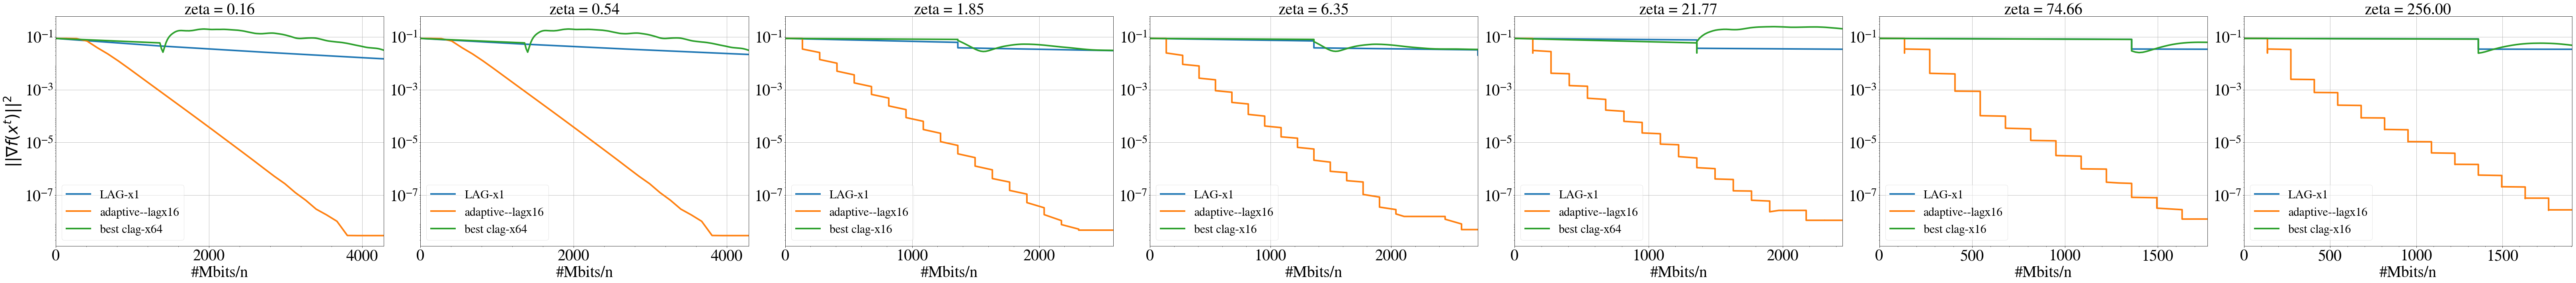
\includegraphics[width=\textwidth]{plots/adaptive/n1.png}
	\caption{Analysis for 1 client. Comparison of convergence between LAG, CLAG, adaptive stepsize LAG}
	\label{fig:anna-100-nodes-grads_main}
\end{figure*}

\begin{figure*}[!h]
	\centering
	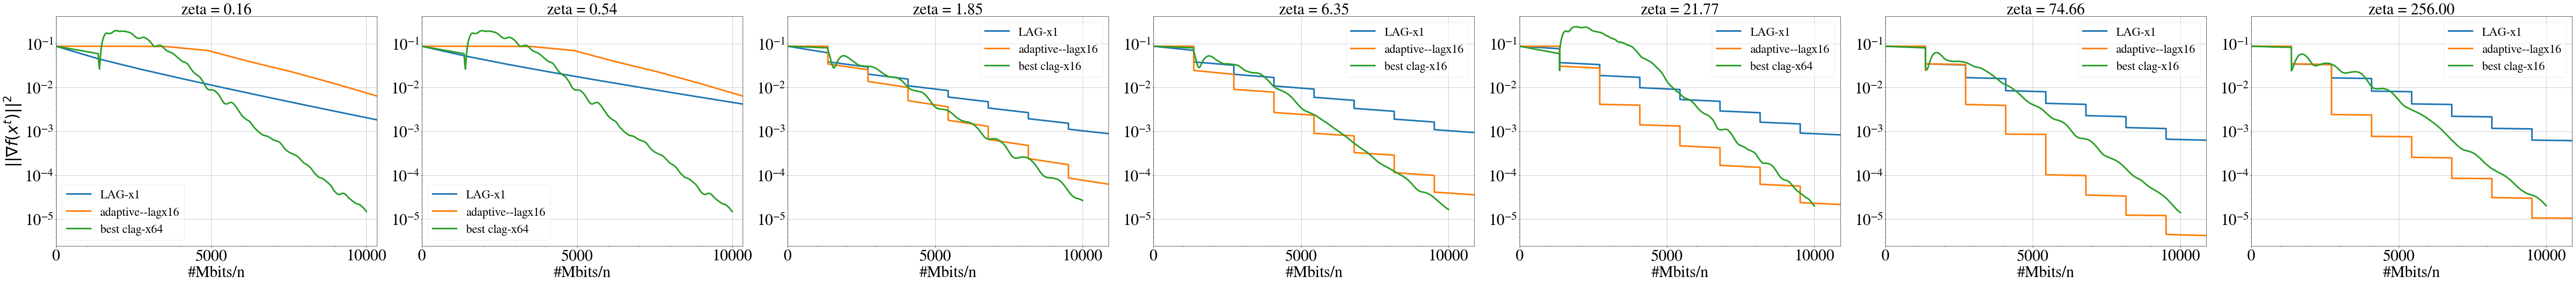
\includegraphics[width=\textwidth]{plots/adaptive/n20.png}
	\caption{Analysis for 20 clients. Comparison of convergence between LAG, CLAG, adaptive stepsize LAG}
	\label{fig:anna-100-nodes-grads_main}
\end{figure*}

\begin{figure*}[!h]
	\centering
	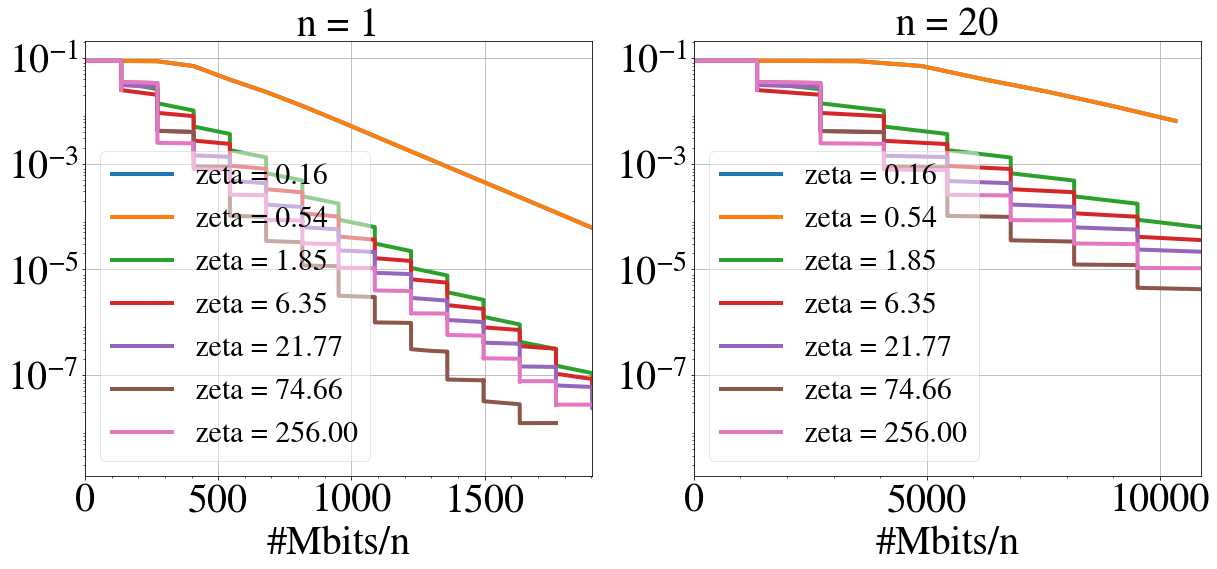
\includegraphics[width=\textwidth]{plots/adaptive/n1_20.png}
	\caption{Analysis for 1 and 20 clients. Comparison of convergence between adaptive LAG with different triggers. }
	\label{fig:anna-100-nodes-grads_main}
\end{figure*}

\clearpage

\subsection{Probabilistic adaptation}

\begin{eqnarray}\label{eq:b_marina_compressor}
\cC_{h,y}(x) = \begin{cases}x,& \text{w.p.\ } 1 - \min\left\{1, \zeta\frac{\sqnorm{x - y}}{\sqnorm{x-h}}\right\}\\ h + \cC(x - h),& \text{w.p.\ } \min\left\{1, \zeta\frac{\sqnorm{x - y}}{\sqnorm{x-h}}\right\} \end{cases}
\end{eqnarray} 

% \begin{figure*}[!h]
% 	\centering
% 	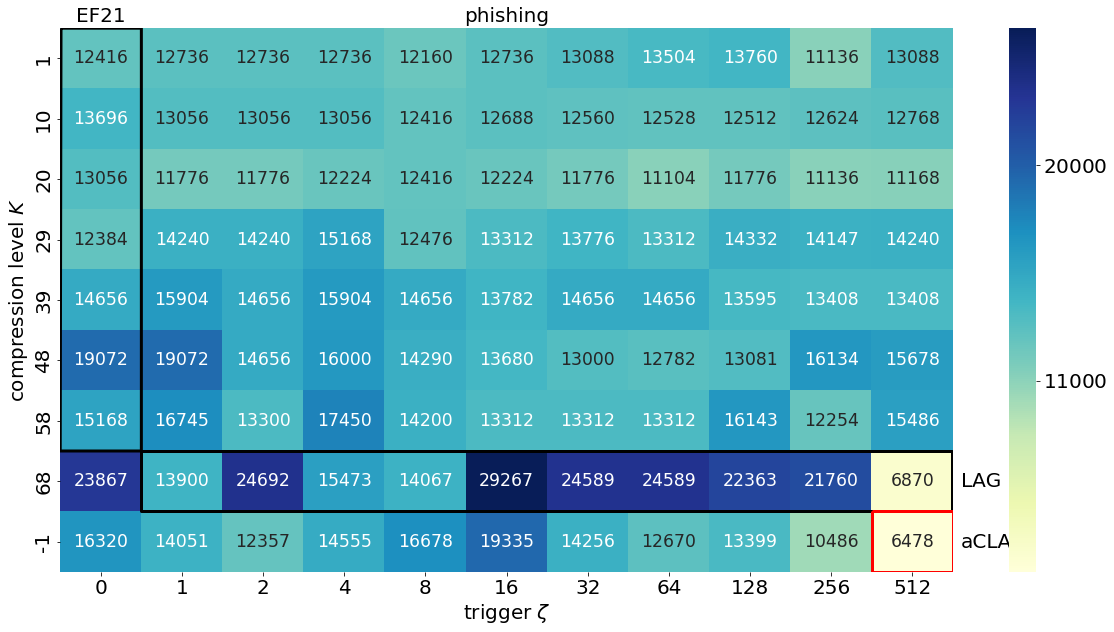
\includegraphics[width=\textwidth]{plots/adaptive/cmap.png}
% 	\caption{(top) Comparison of different \algname{3PC} Top-$K$ compressors. $\zeta = 0.16$, phishing dataset. (bottom) Distribution  of different communication mechanisms used during the training by different optimizers.}
% 	\label{fig:anna-100-nodes-grads_main}
% \end{figure*}

\begin{figure*}[!h]
	\centering
	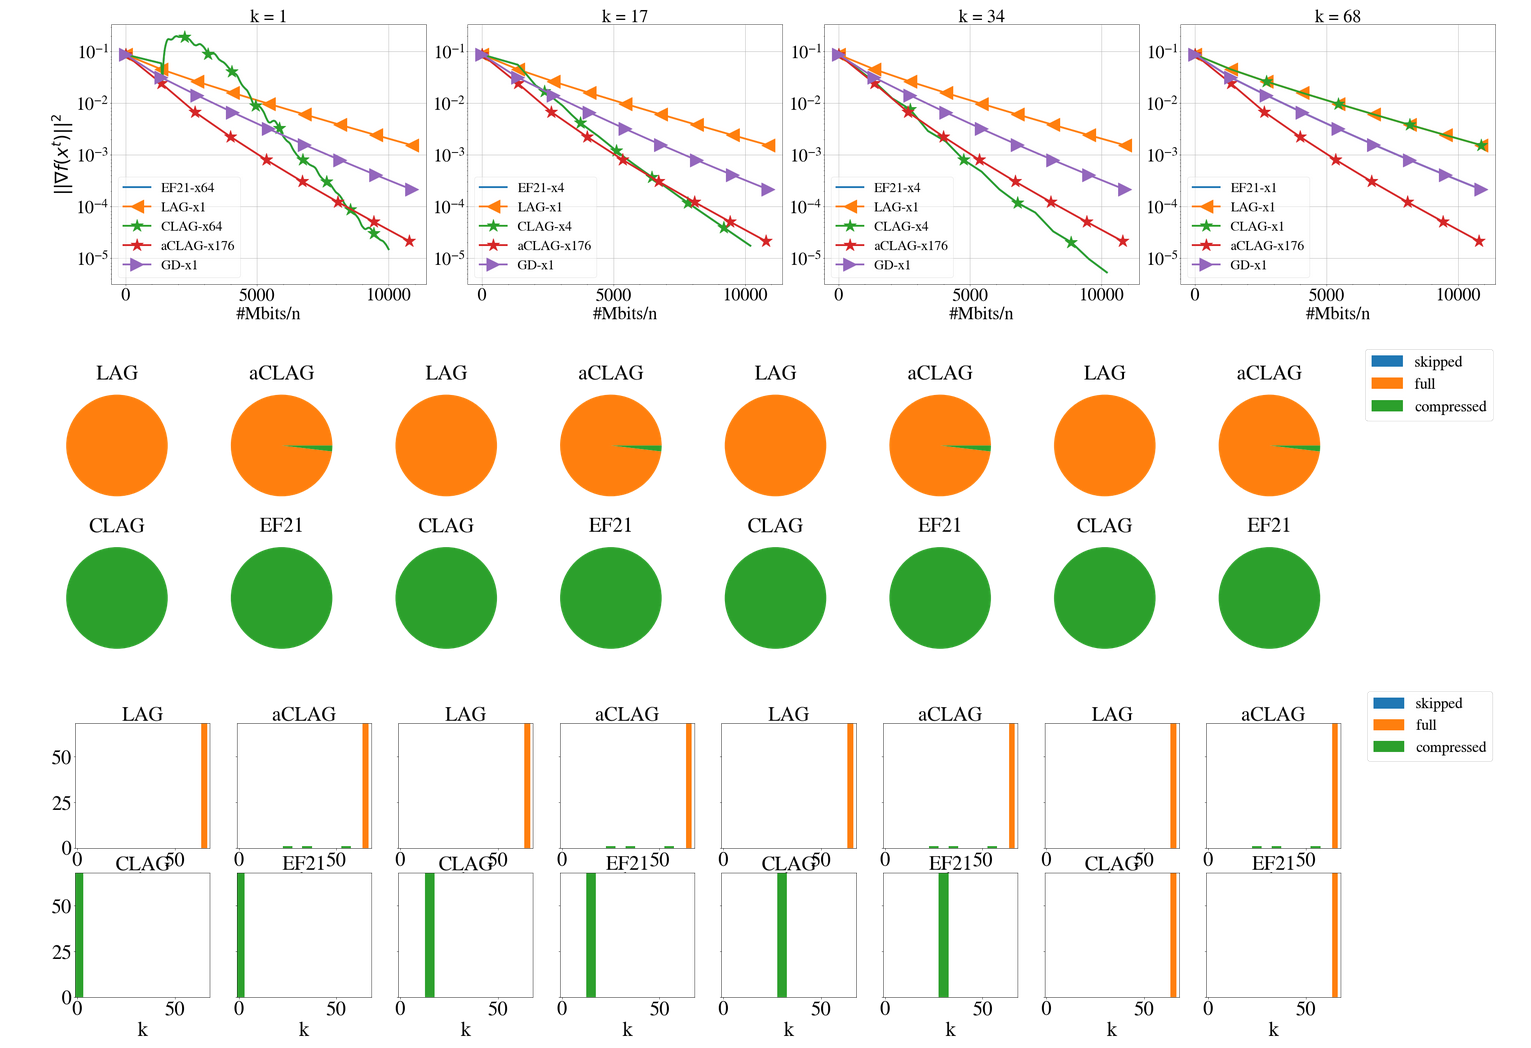
\includegraphics[width=\textwidth]{plots/adaptive/old_4.png}
	\caption{Analysis for 20 clients. (top) Comparison of different \algname{3PC} Top-$K$ compressors. $\zeta = 0.16$, phishing dataset. (bottom) Distribution  of different communication mechanisms used during the training by different optimizers.}
	\label{fig:anna-100-nodes-grads_main}
\end{figure*}

\begin{figure*}[!h]
	\centering
	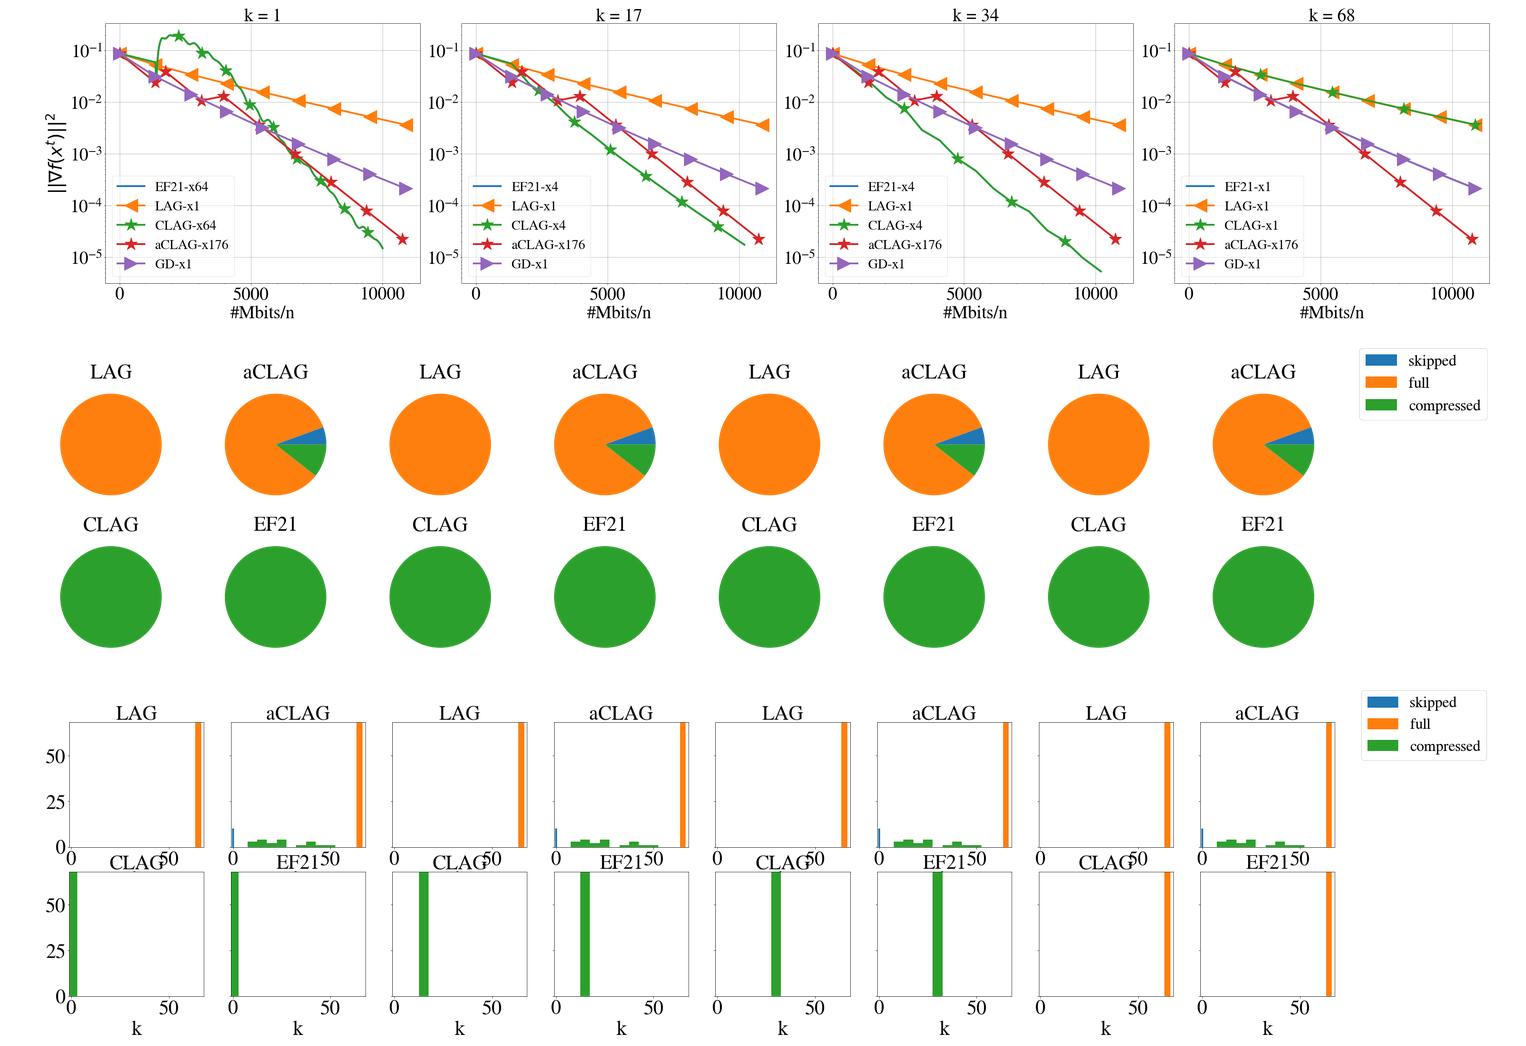
\includegraphics[width=\textwidth]{plots/adaptive/old_5.png}
	\caption{Analysis for 20 clients. (top) Comparison of different \algname{3PC} Top-$K$ compressors. $\zeta = 1.85$, phishing dataset. (bottom) Distribution  of different communication mechanisms used during the training by different optimizers.}
	\label{fig:anna-100-nodes-grads_main}
\end{figure*}

\begin{figure*}[!h]
	\centering
	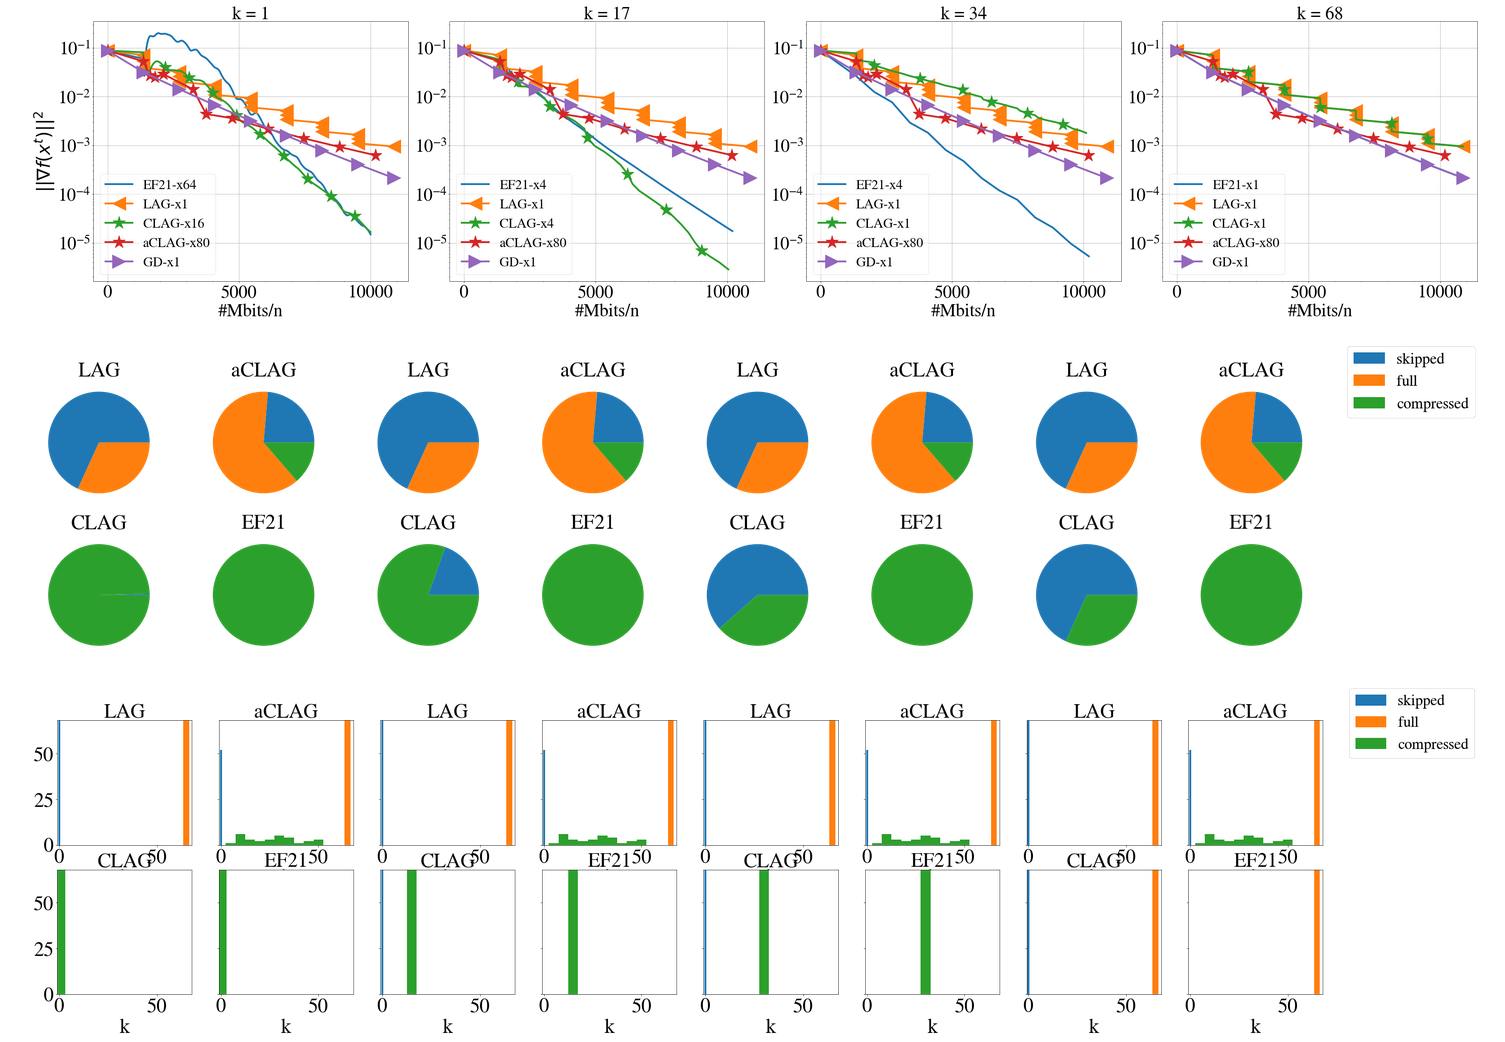
\includegraphics[width=\textwidth]{plots/adaptive/old_7.png}
	\caption{Analysis for 20 clients. (top) Comparison of different \algname{3PC} Top-$K$ compressors. $\zeta = 22$, phishing dataset. (bottom) Distribution  of different communication mechanisms used during the training by different optimizers.}
	\label{fig:anna-100-nodes-grads_main}
\end{figure*}

\begin{figure*}[!h]
	\centering
	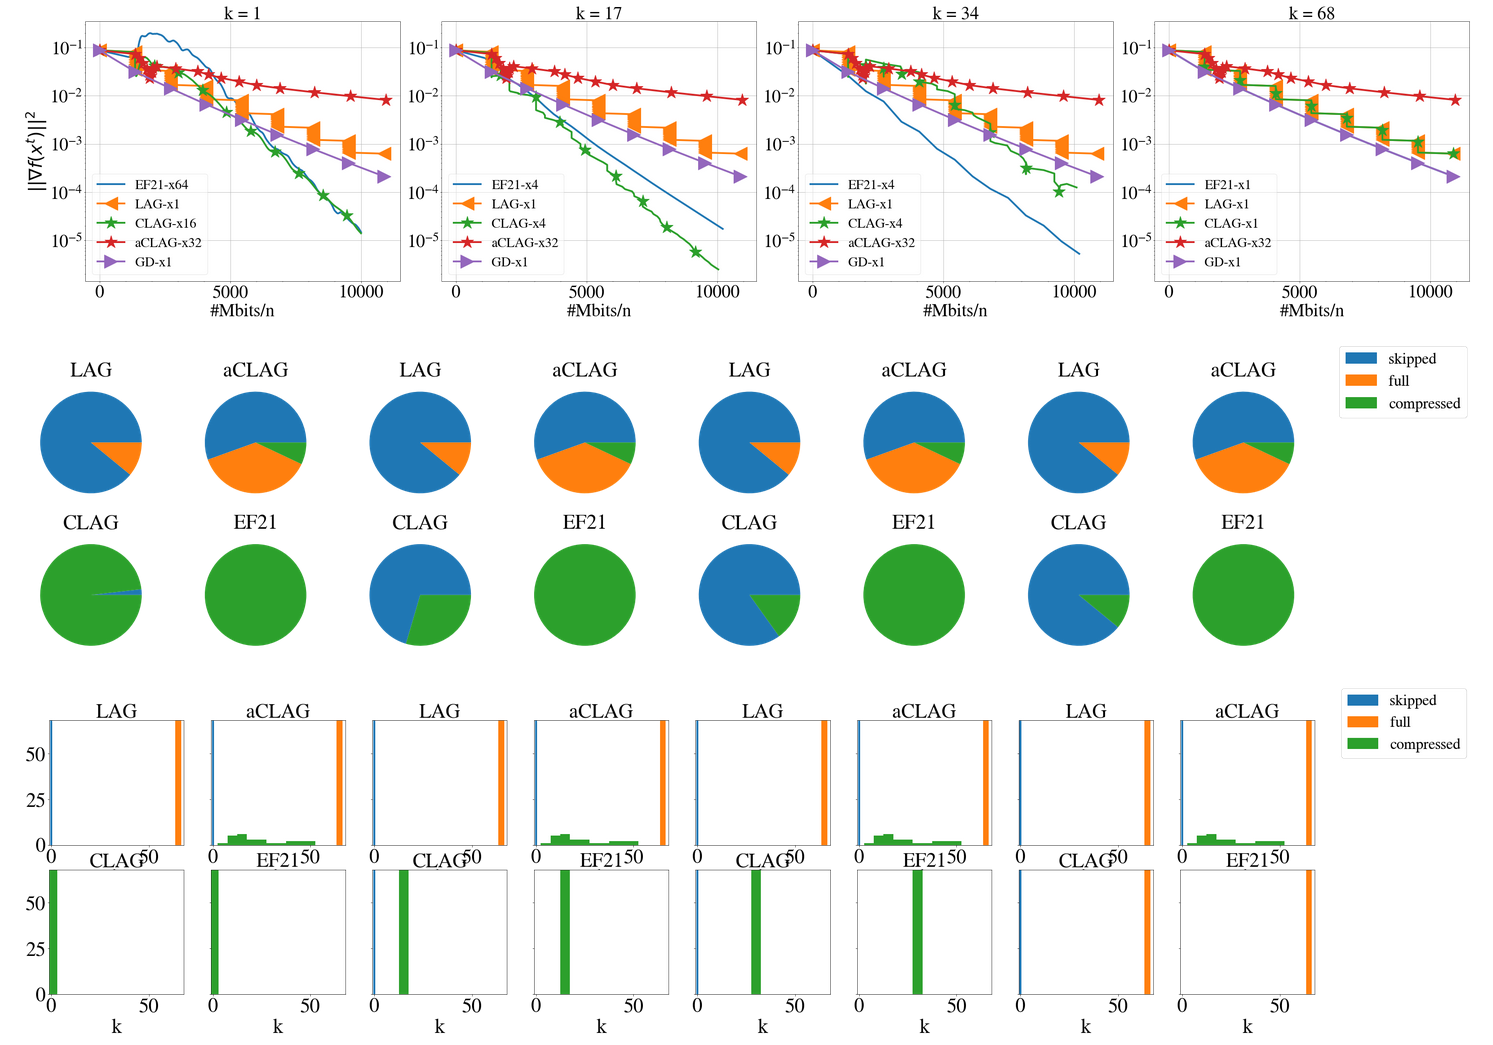
\includegraphics[width=\textwidth]{plots/adaptive/old_9.png}
	\caption{Analysis for 20 clients. (top) Comparison of different \algname{3PC} Top-$K$ compressors. $\zeta = 256$, phishing dataset. (bottom) Distribution  of different communication mechanisms used during the training by different optimizers.}
	\label{fig:anna-100-nodes-grads_main}
\end{figure*}

\begin{figure*}[!h]
	\centering
	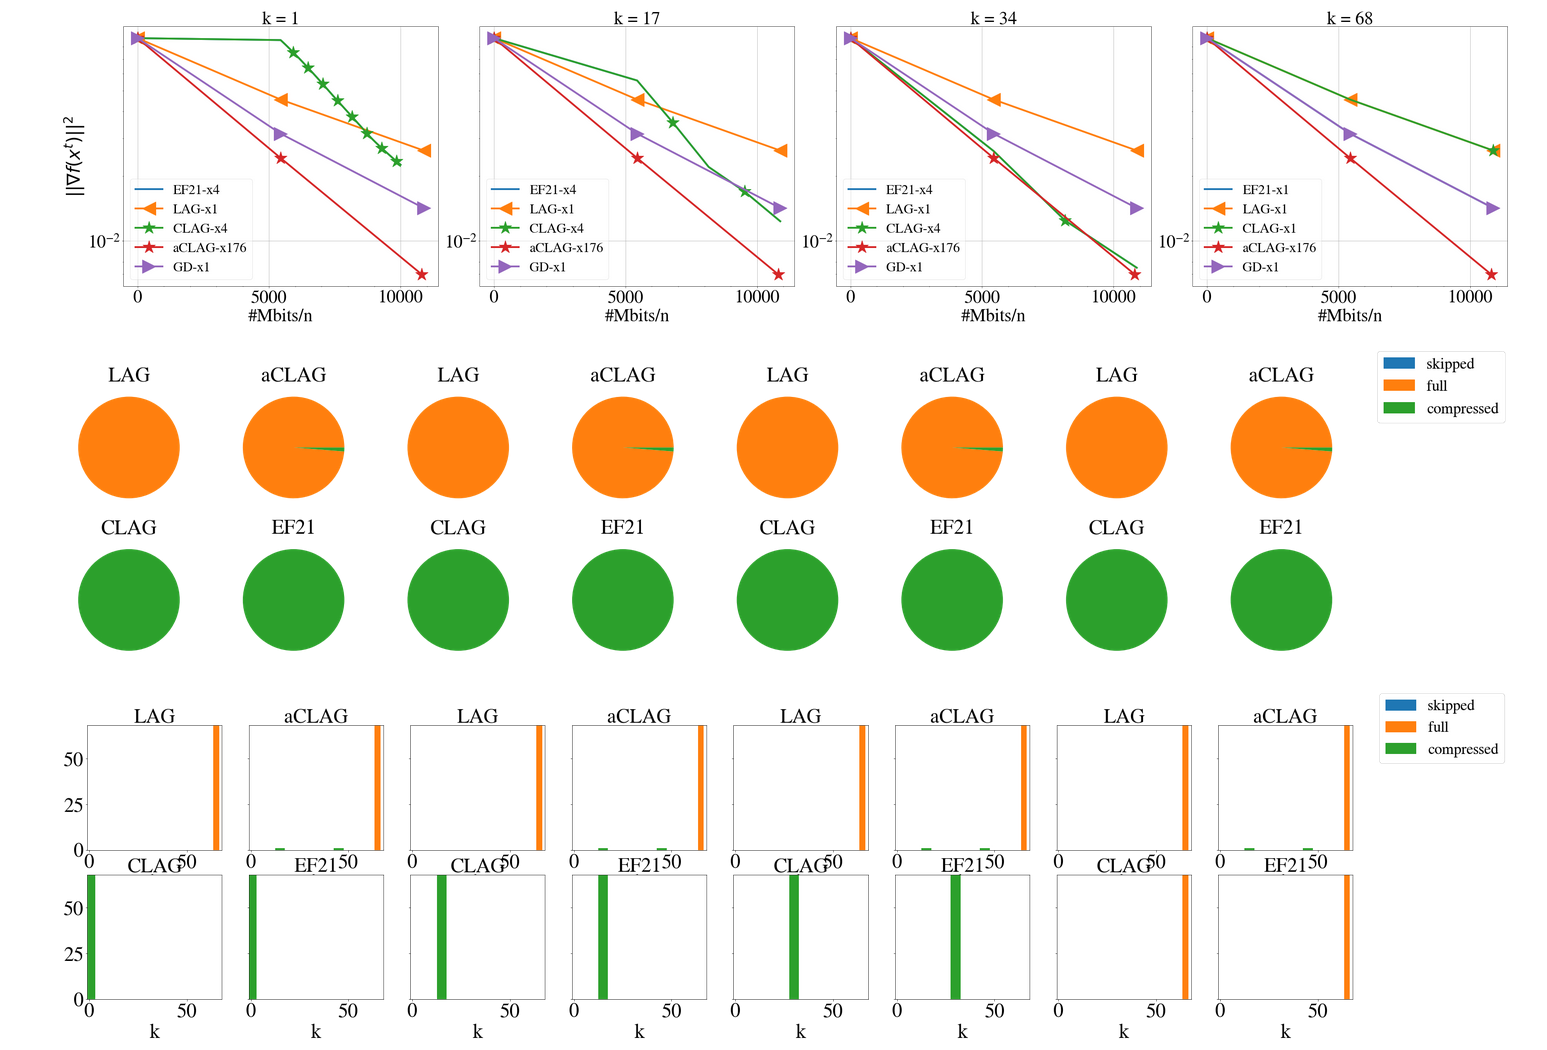
\includegraphics[width=\textwidth]{plots/adaptive/new_4.png}
	\caption{Analysis for 80 clients. (top) Comparison of different \algname{3PC} Top-$K$ compressors. $\zeta = 0.16$, phishing dataset. (bottom) Distribution  of different communication mechanisms used during the training by different optimizers.}
	\label{fig:anna-100-nodes-grads_main}
\end{figure*}

\begin{figure*}[!h]
	\centering
	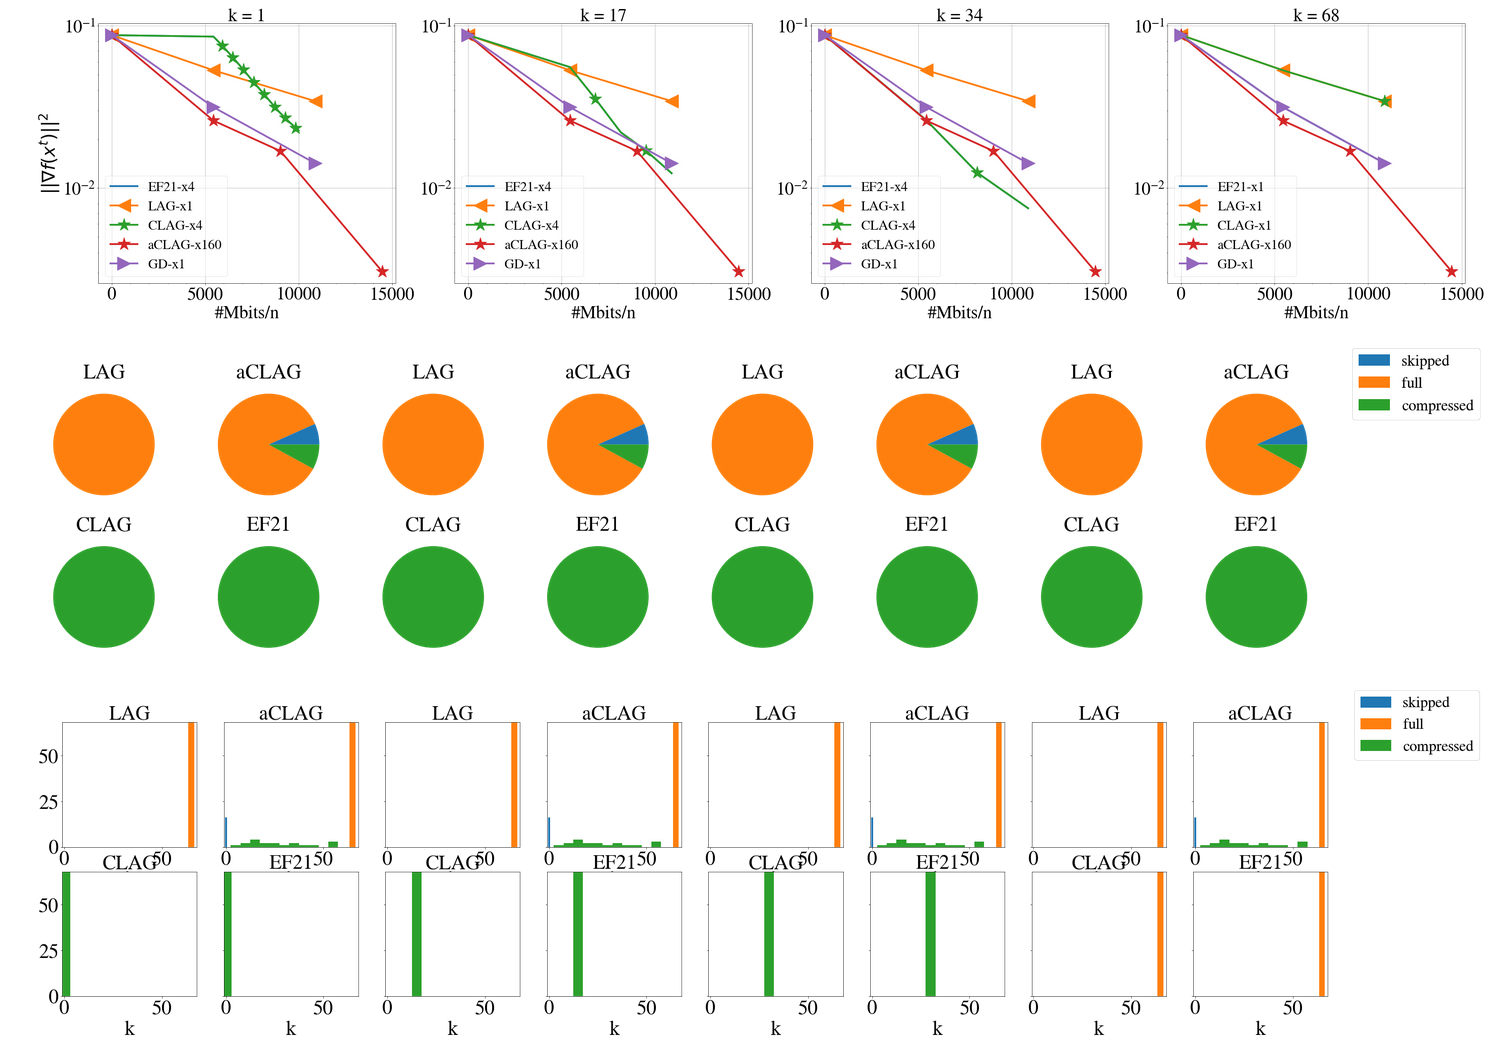
\includegraphics[width=\textwidth]{plots/adaptive/new_5.png}
	\caption{Analysis for 80 clients. (top) Comparison of different \algname{3PC} Top-$K$ compressors. $\zeta = 1.85$, phishing dataset. (bottom) Distribution  of different communication mechanisms used during the training by different optimizers.}
	\label{fig:anna-100-nodes-grads_main}
\end{figure*}


\begin{figure*}[!h]
	\centering
	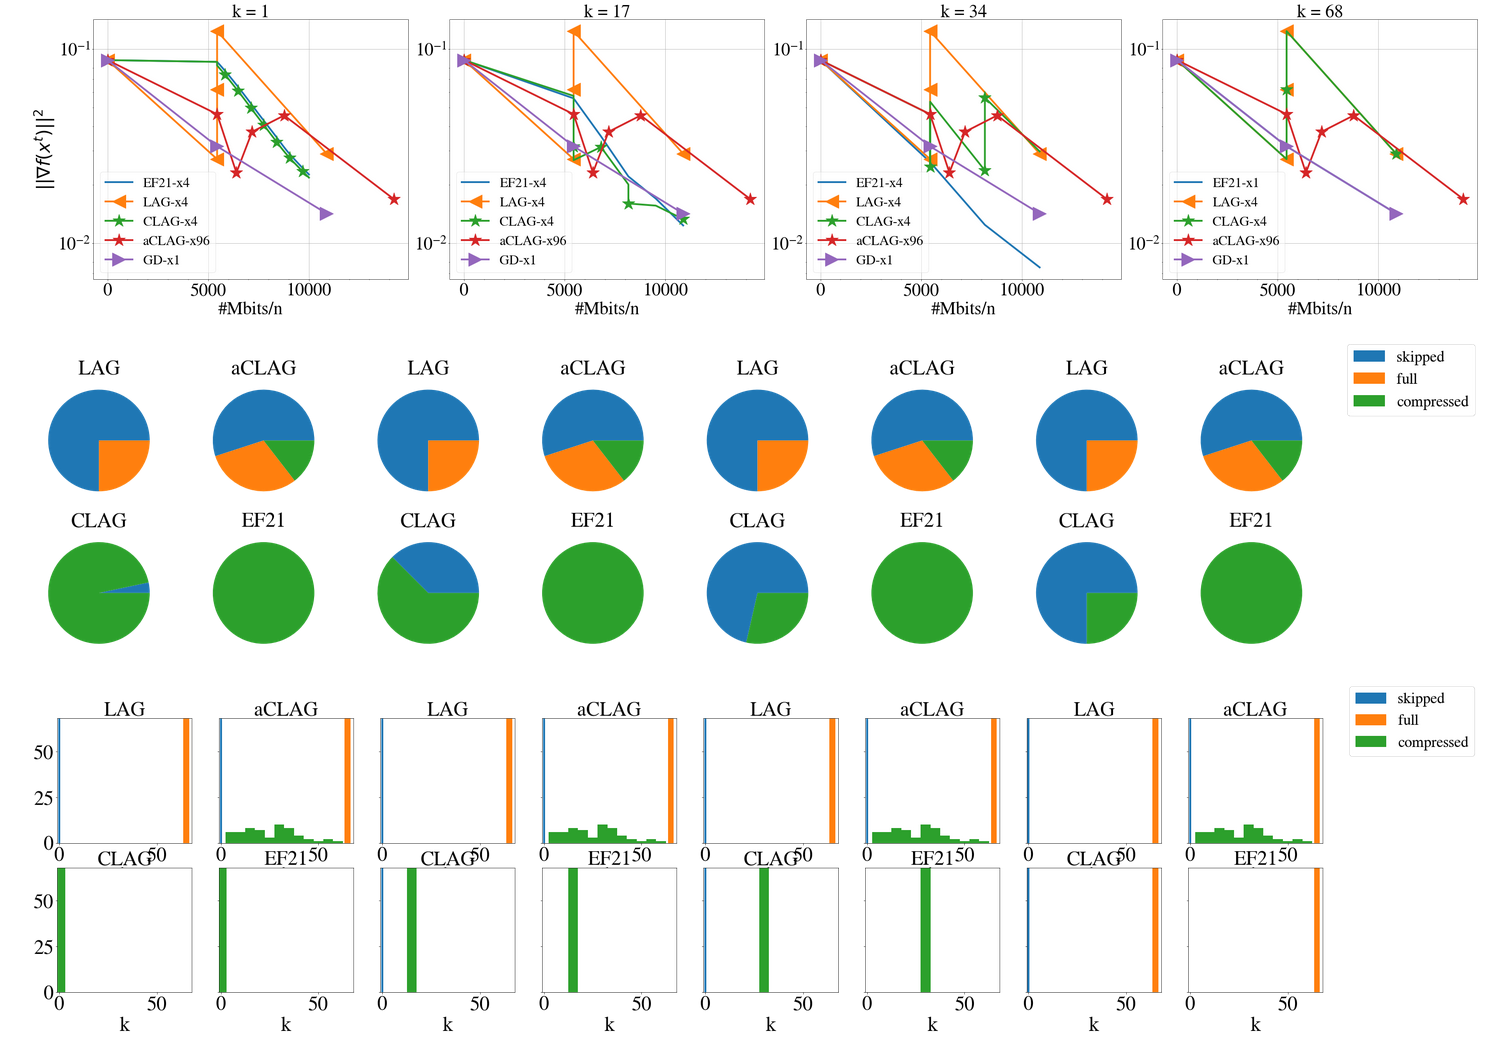
\includegraphics[width=\textwidth]{plots/adaptive/new_7.png}
	\caption{Analysis for 80 clients. (top) Comparison of different \algname{3PC} Top-$K$ compressors. $\zeta = 22$, phishing dataset. (bottom) Distribution  of different communication mechanisms used during the training by different optimizers.}
	\label{fig:anna-100-nodes-grads_main}
\end{figure*}

\begin{figure*}[!h]
	\centering
	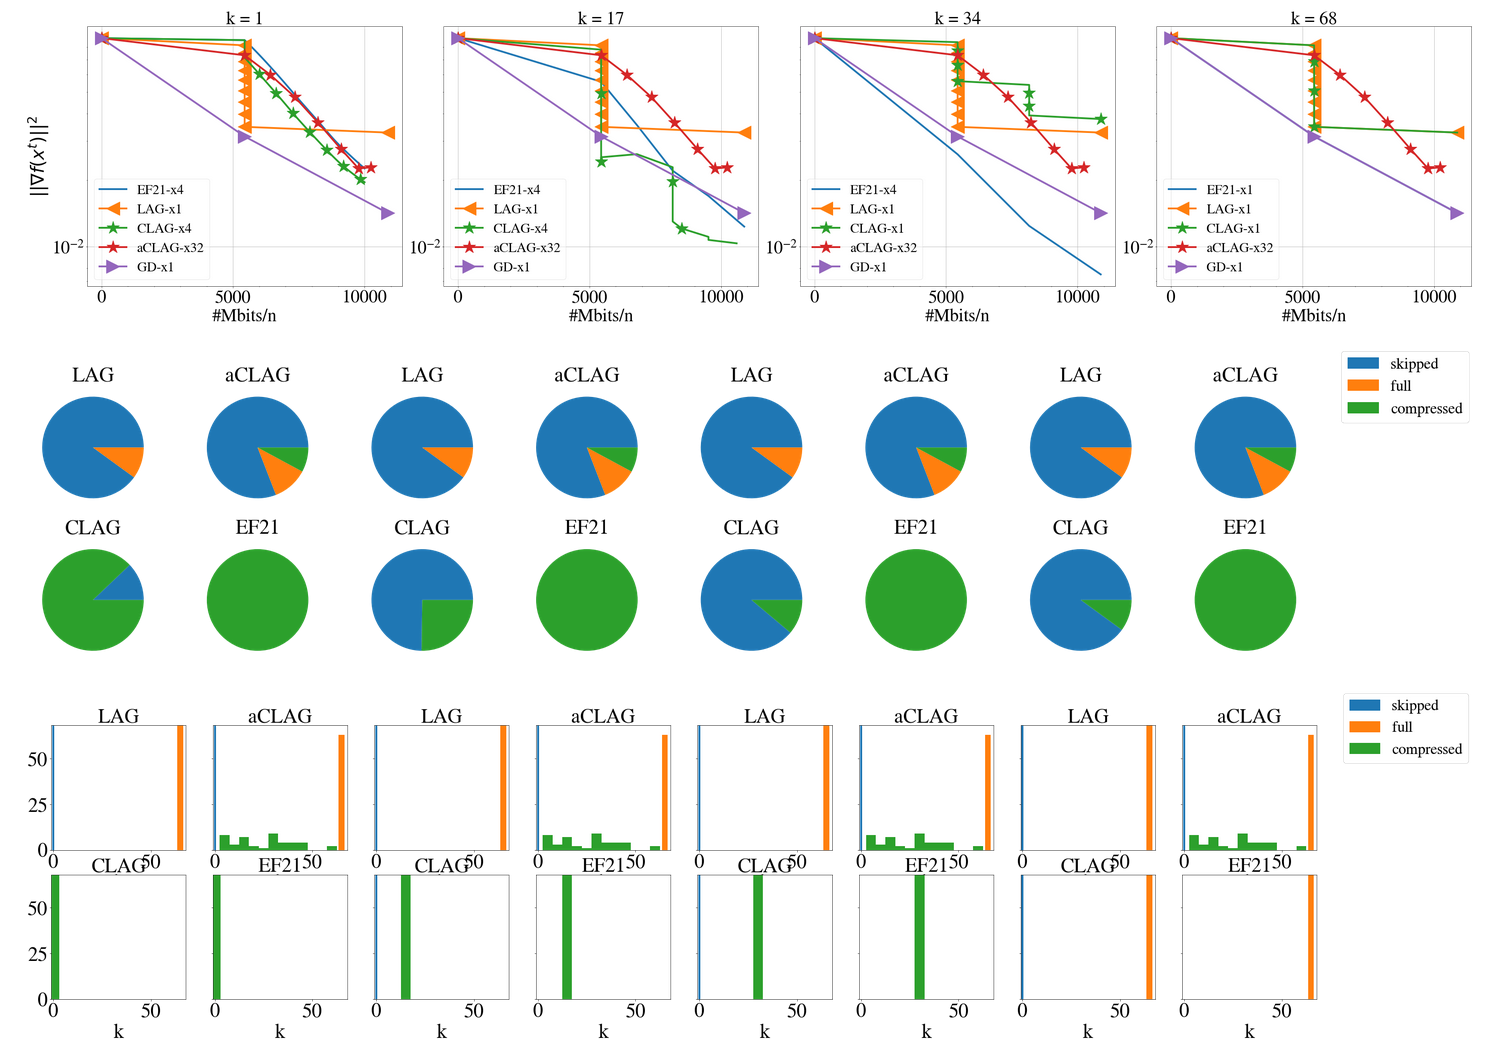
\includegraphics[width=\textwidth]{plots/adaptive/new_9.png}
	\caption{Analysis for 80 clients. (top) Comparison of different \algname{3PC} Top-$K$ compressors. $\zeta = 256$, phishing dataset. (bottom) Distribution  of different communication mechanisms used during the training by different optimizers.}
	\label{fig:anna-100-nodes-grads_main}
\end{figure*}

\begin{figure*}[!h]
	\centering
	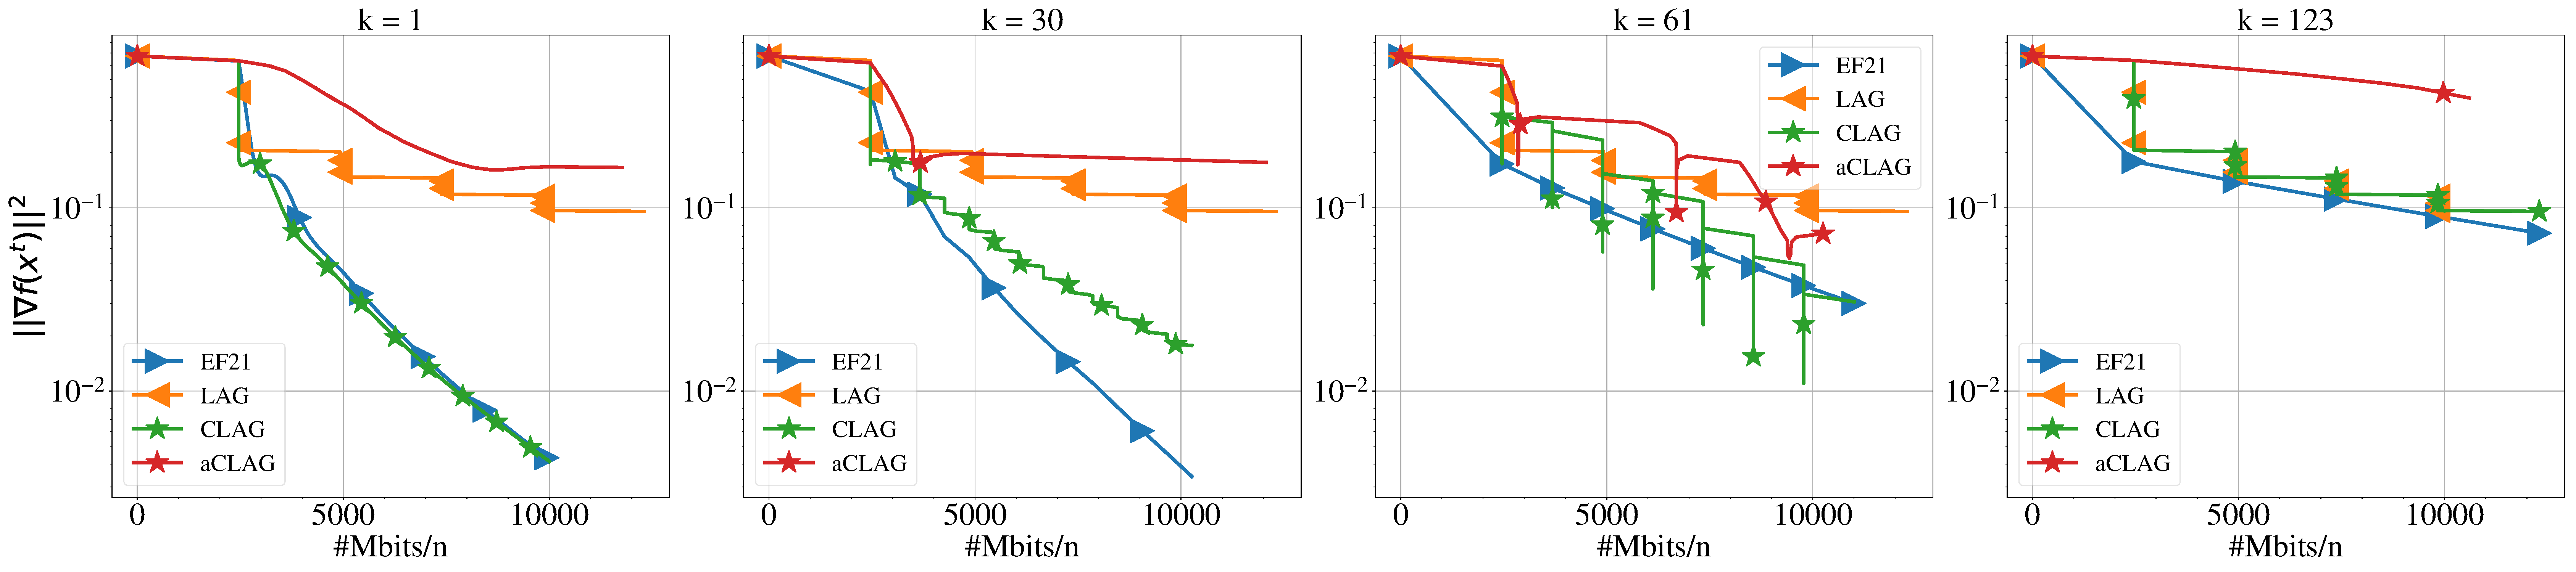
\includegraphics[width=\textwidth]{plots/adaptive/plot_a9a_256.0.pdf}
	\caption{Comparison of different \algname{3PC} Top-$K$ compressors. $\zeta = 256$, a9a dataset}
	\label{fig:anna-100-nodes-grads_main}
\end{figure*}

\begin{figure*}[!h]
	\centering
	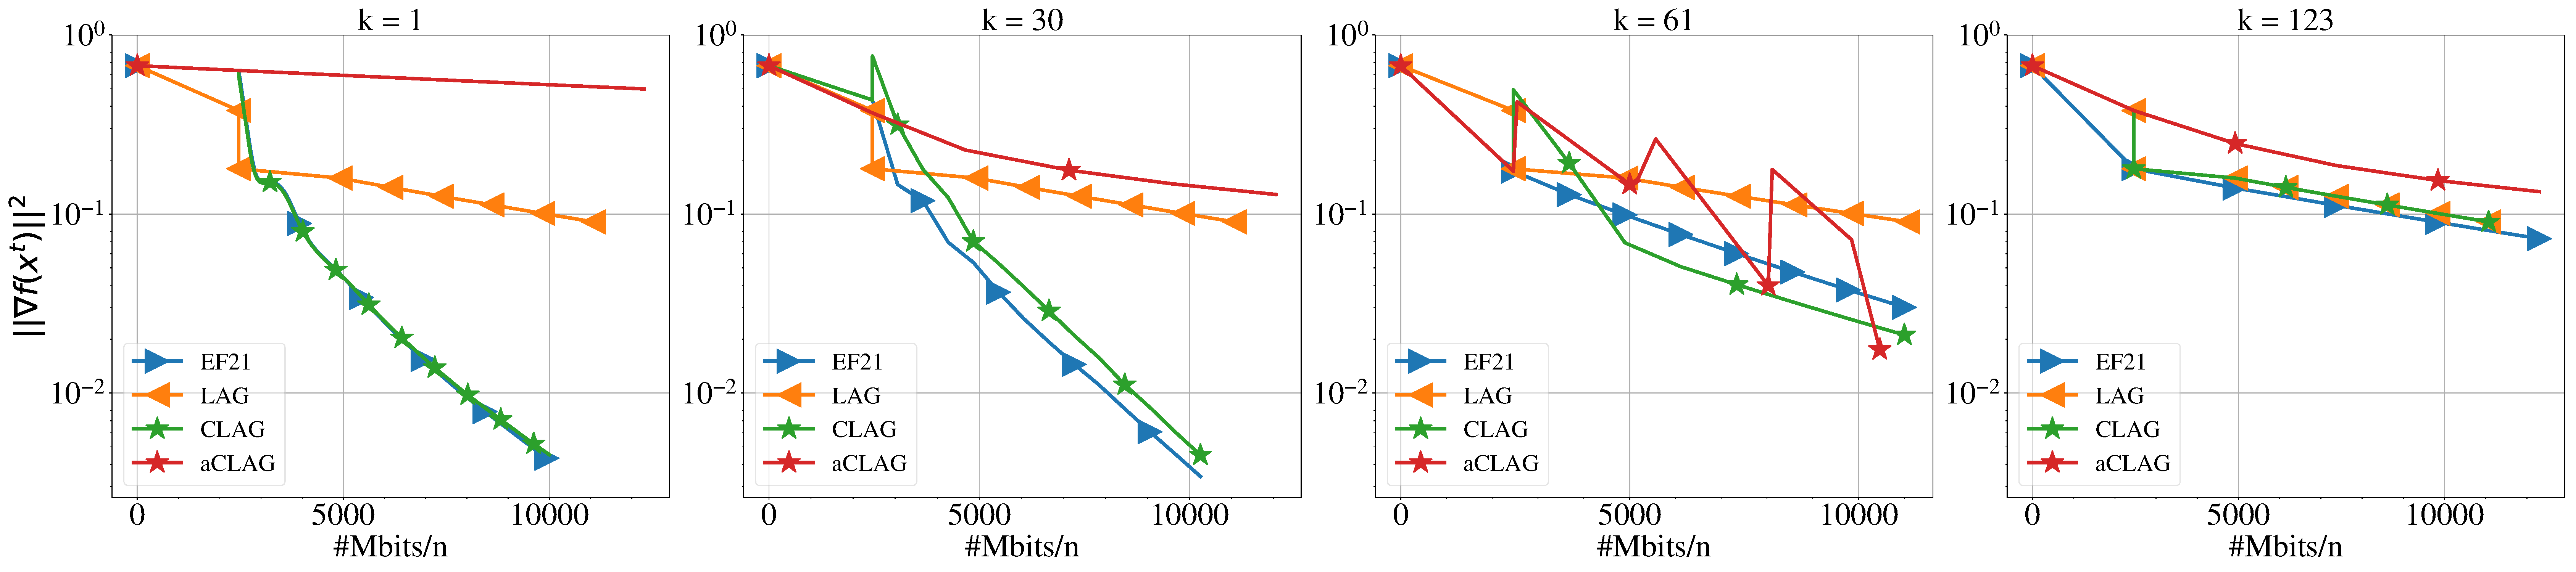
\includegraphics[width=\textwidth]{plots/adaptive/plot_a9a_1.0.pdf}
	\caption{Comparison of different \algname{3PC} Top-$K$ compressors. $\zeta = 1.0$, a9a dataset}
	\label{fig:anna-100-nodes-grads_main}
\end{figure*}

\begin{figure*}[!h]
	\centering
	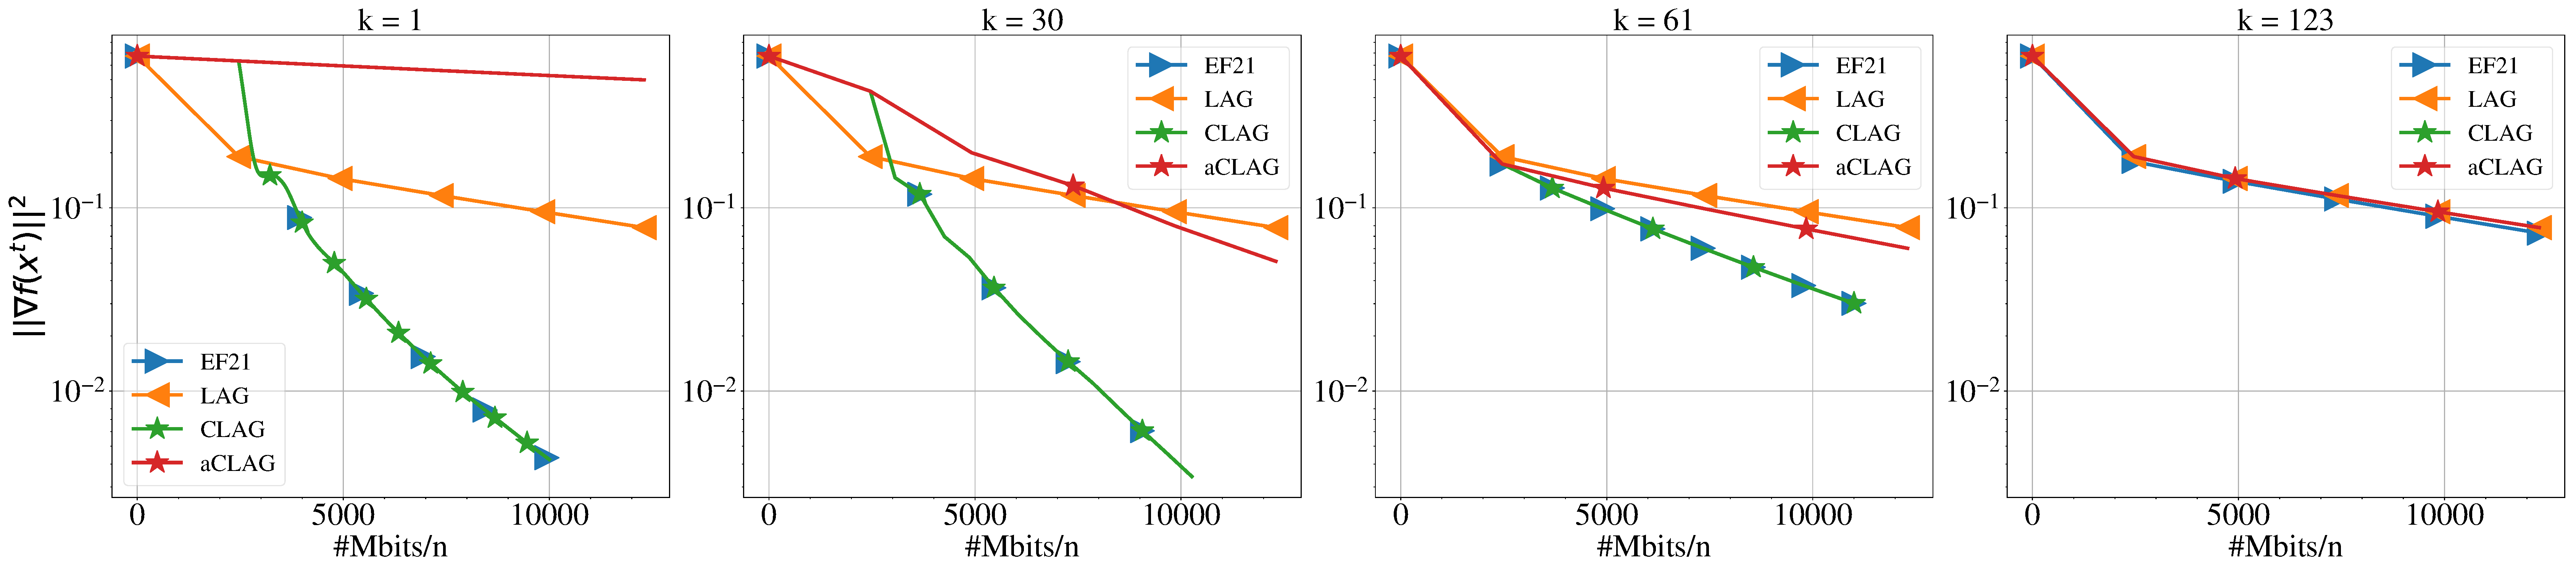
\includegraphics[width=\textwidth]{plots/adaptive/plot_a9a_0.0039.pdf}
	\caption{Comparison of different \algname{3PC} Top-$K$ compressors.  $\zeta = 0.0039$, a9a dataset}
	\label{fig:anna-100-nodes-grads_main}
\end{figure*}

\begin{figure*}[!h]
	\centering
	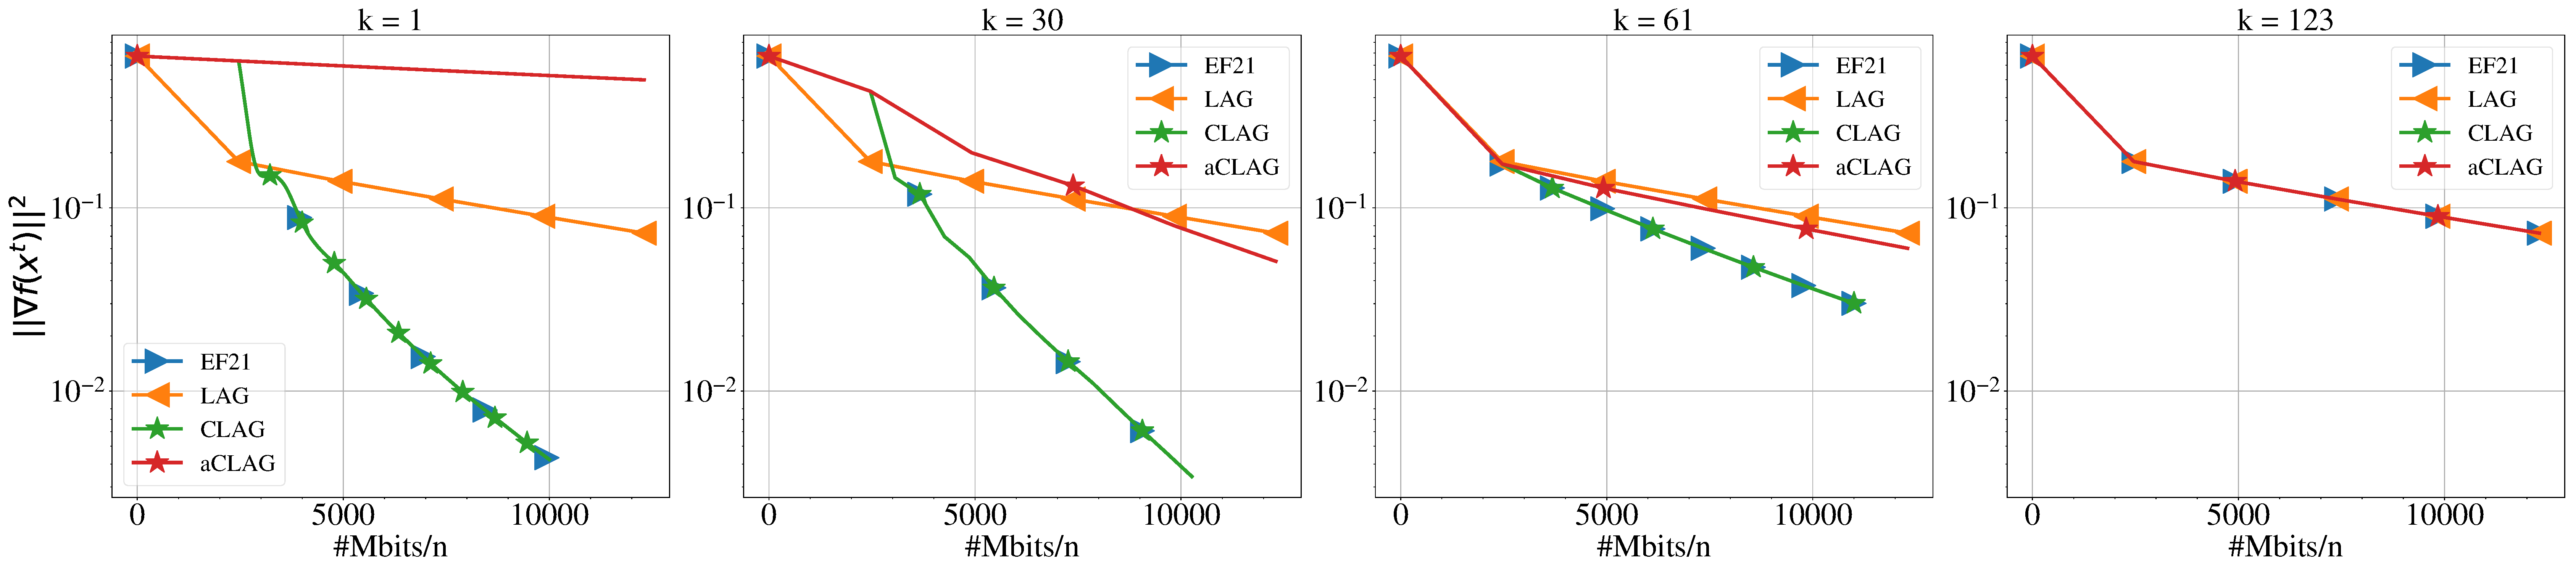
\includegraphics[width=\textwidth]{plots/adaptive/plot_a9a_0.0.pdf}
	\caption{Comparison of different \algname{3PC} Top-$K$ compressors.$\zeta = 0.0$, a9a dataset}
	\label{fig:anna-100-nodes-grads_main}
\end{figure*}

\newpage

\begin{figure*}[!h]
	\centering
	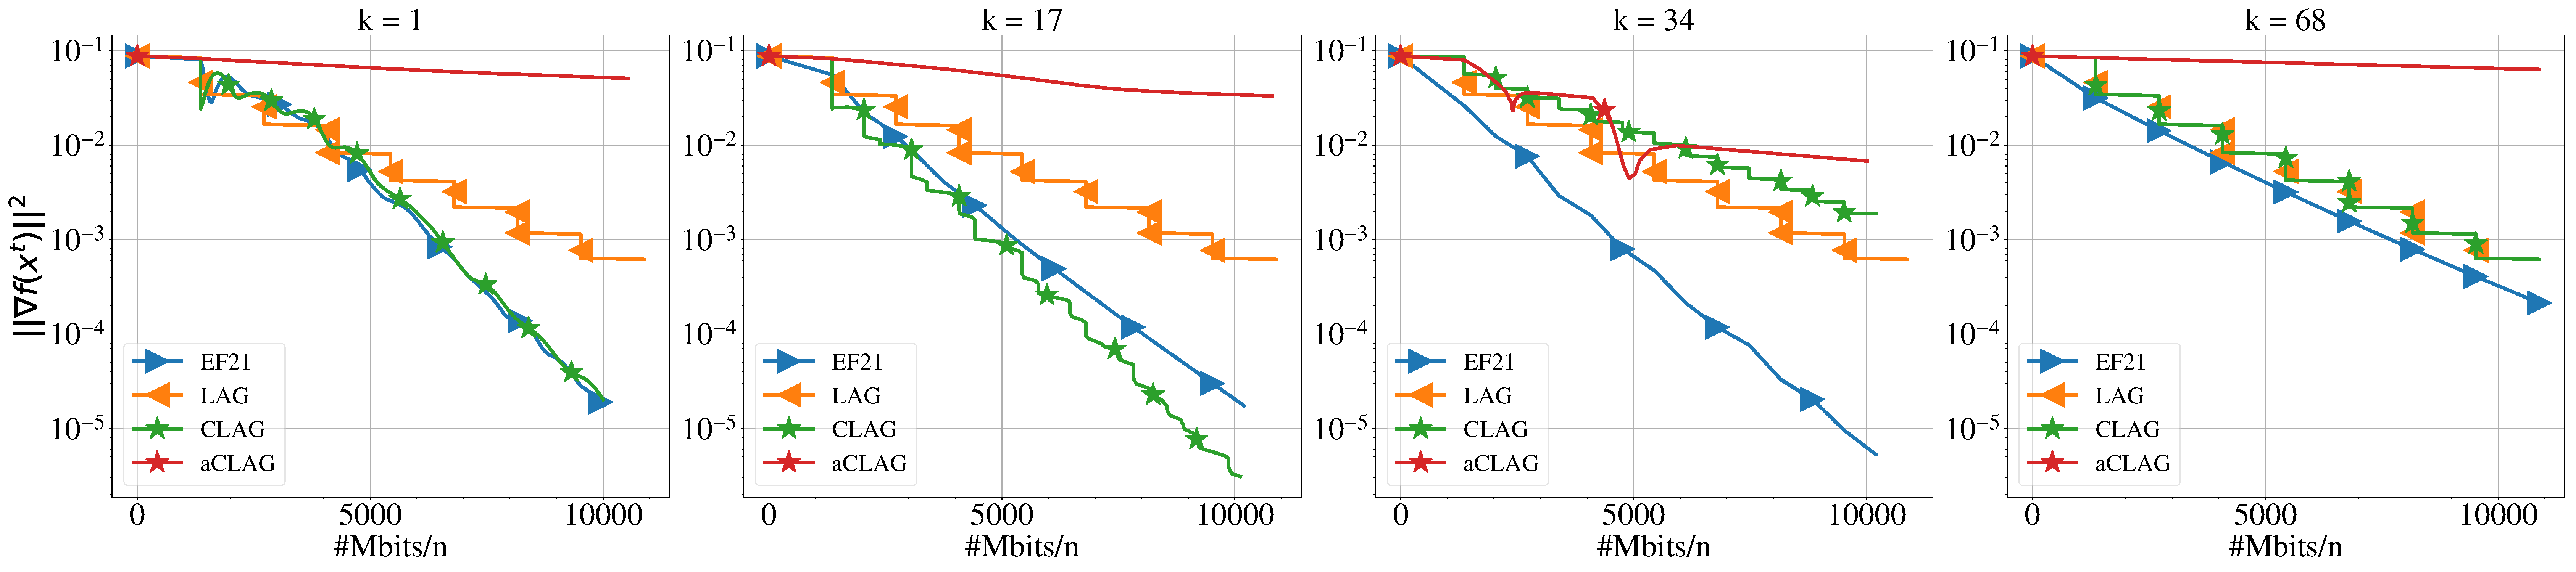
\includegraphics[width=\textwidth]{plots/adaptive/plot_phishing_256.0.pdf}
	\caption{Comparison of different \algname{3PC} Top-$K$ compressors. $\zeta = 256$, phishing dataset}
	\label{fig:anna-100-nodes-grads_main}
\end{figure*}

\begin{figure*}[!h]
	\centering
	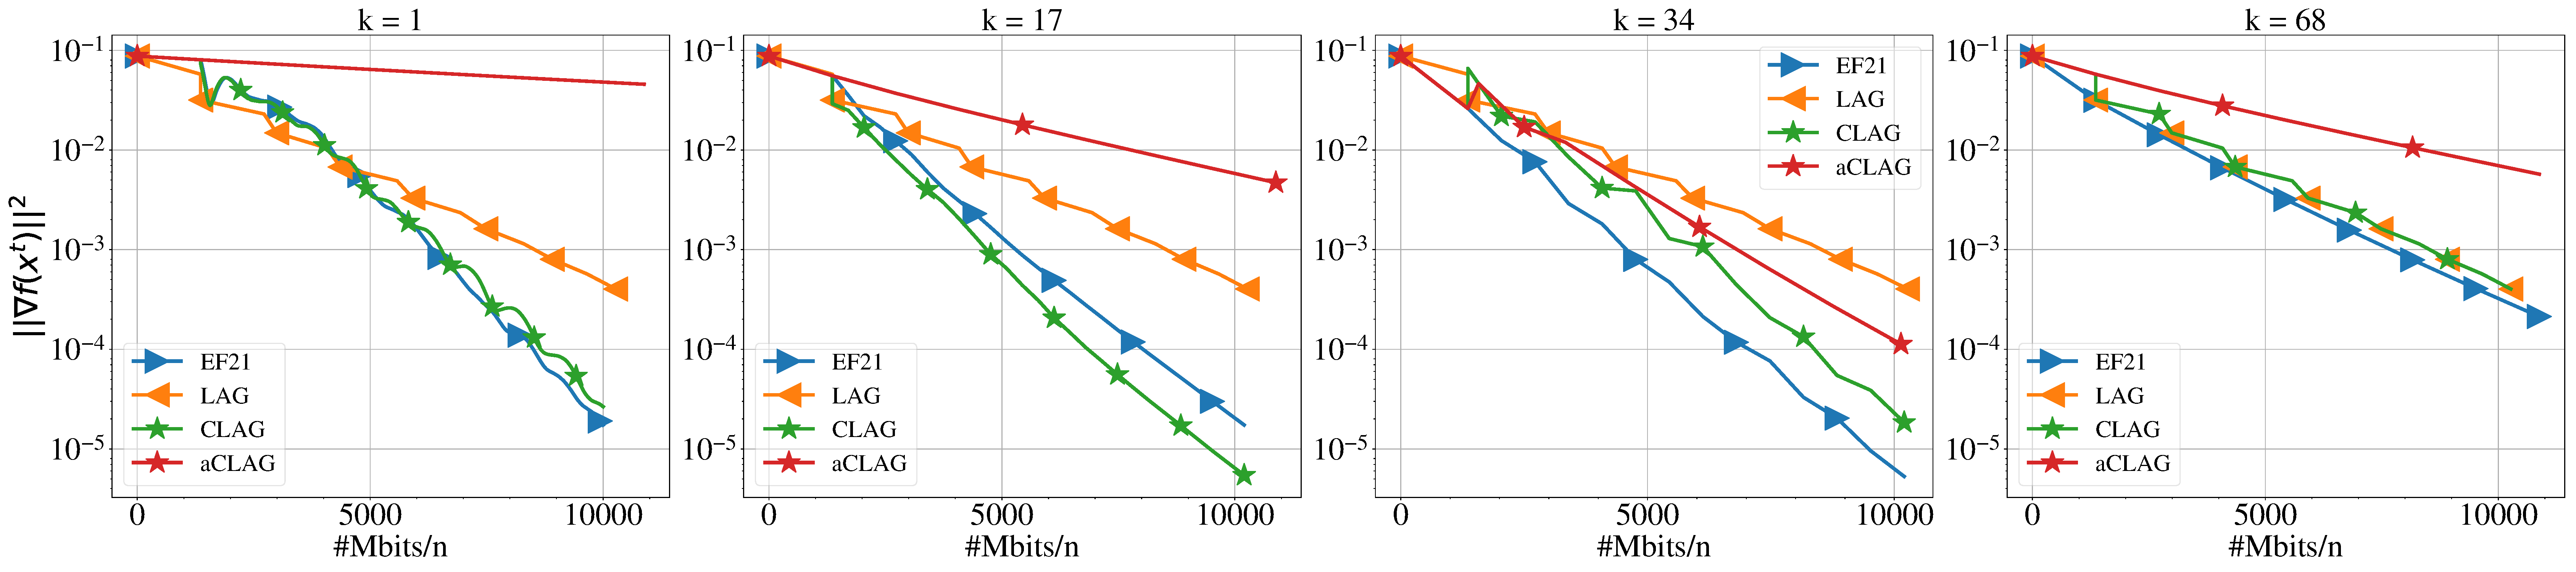
\includegraphics[width=\textwidth]{plots/adaptive/plot_phishing_1.0.pdf}
	\caption{Comparison of different \algname{3PC} Top-$K$ compressors. $\zeta = 1.0$, phishing dataset}
	\label{fig:anna-100-nodes-grads_main}
\end{figure*}

\begin{figure*}[!h]
	\centering
	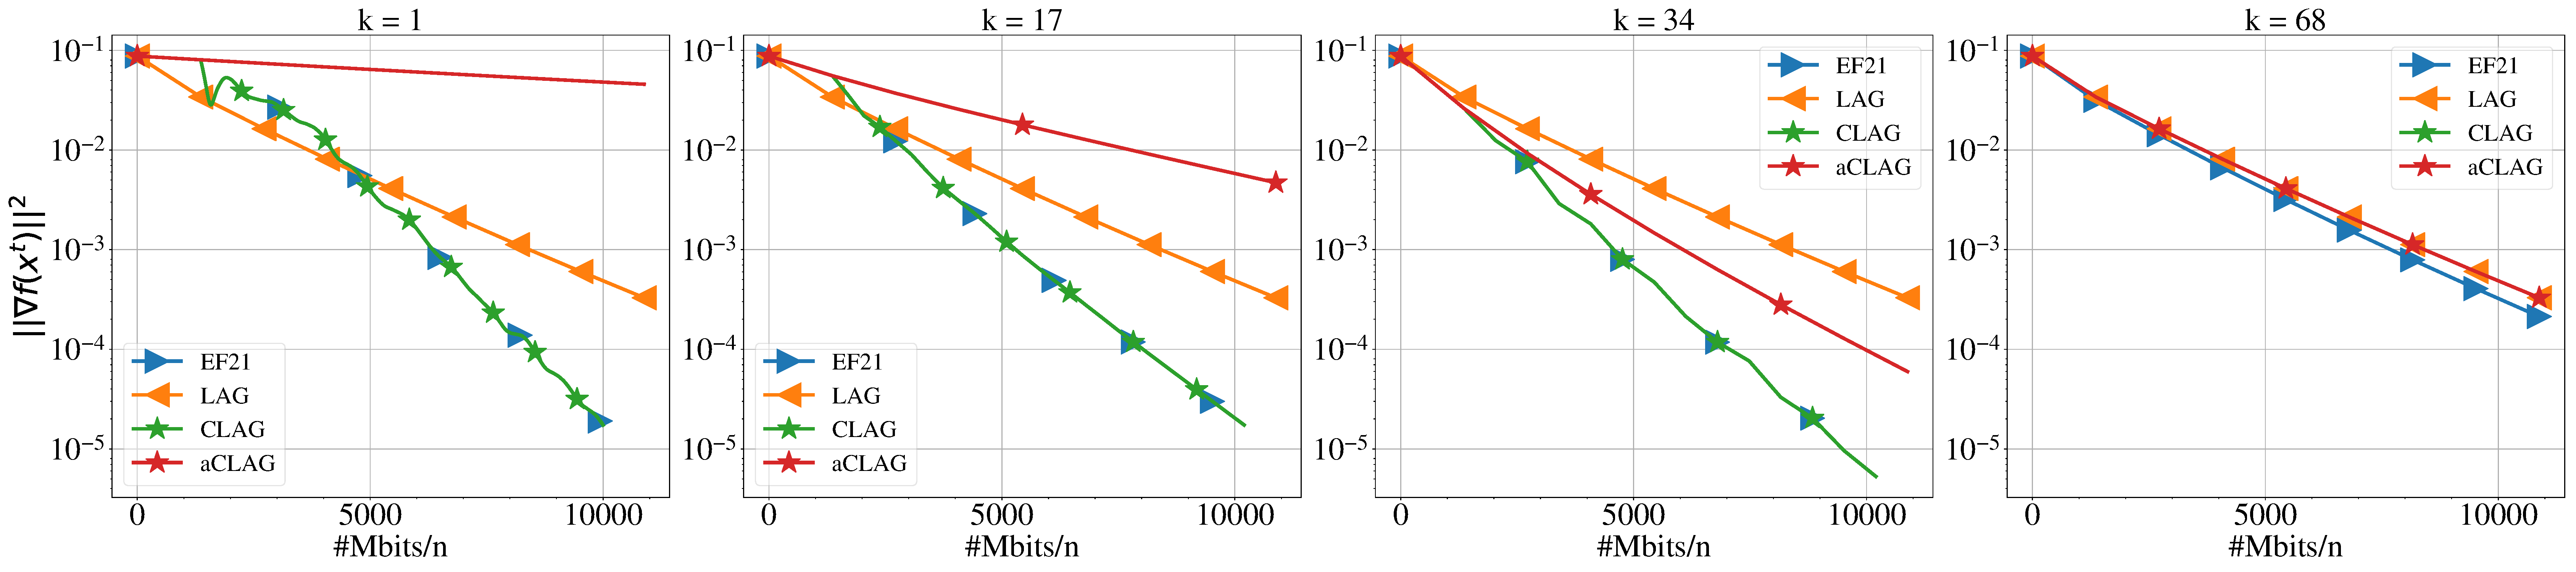
\includegraphics[width=\textwidth]{plots/adaptive/plot_phishing_0.0039.pdf}
	\caption{Comparison of different \algname{3PC} Top-$K$ compressors.  $\zeta = 0.0039$, phishing dataset}
	\label{fig:anna-100-nodes-grads_main}
\end{figure*}

\begin{figure*}[!h]
	\centering
	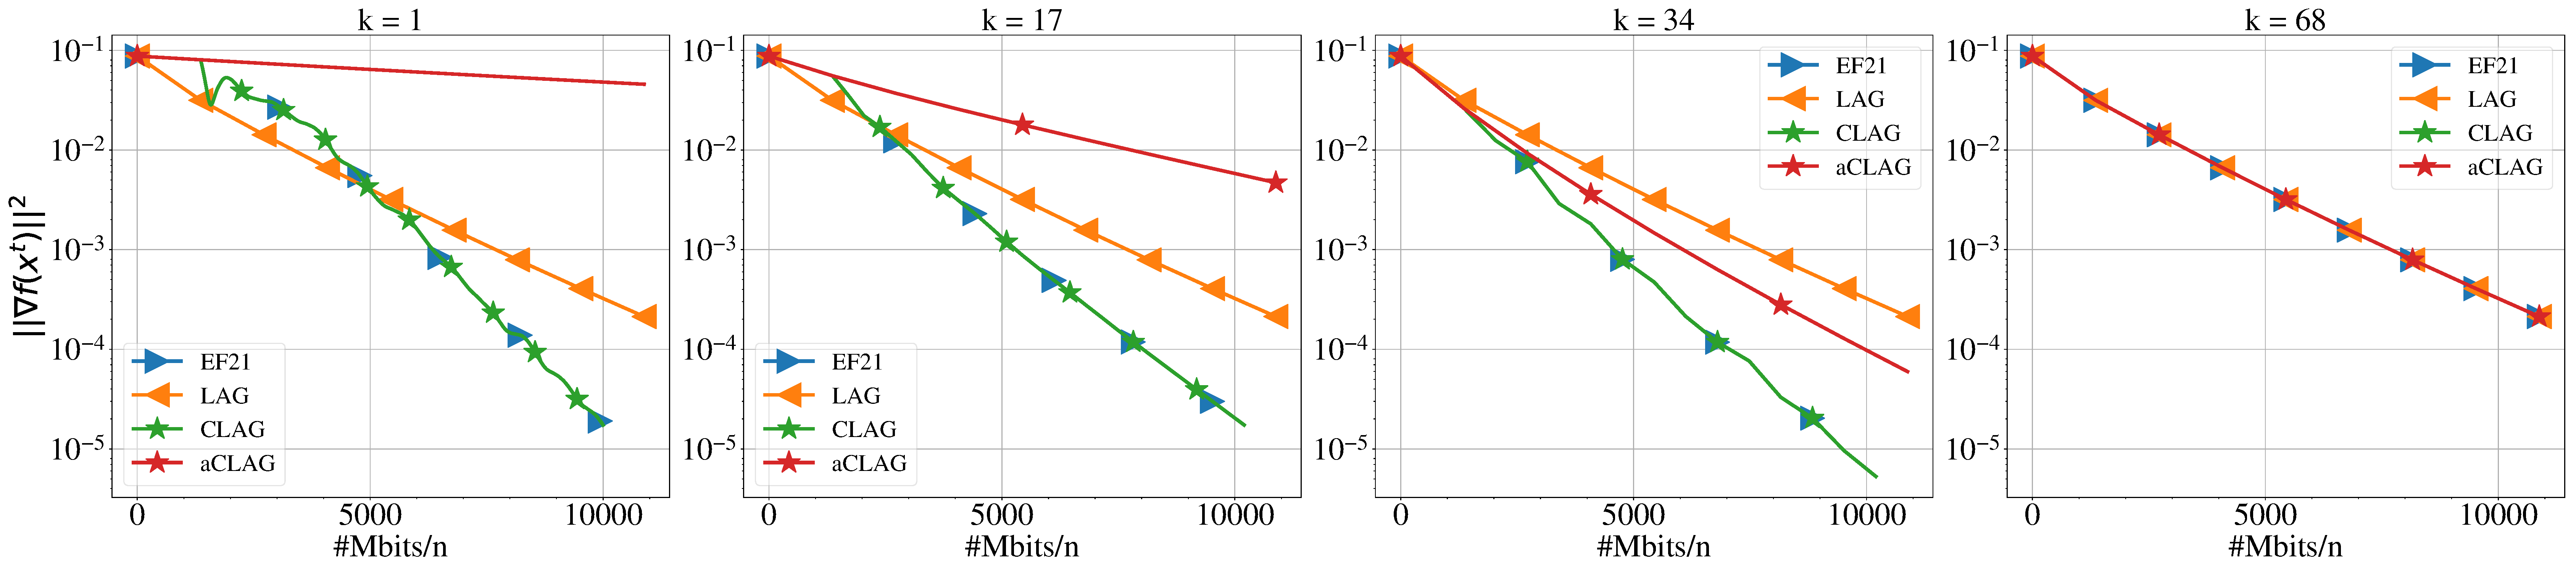
\includegraphics[width=\textwidth]{plots/adaptive/plot_phishing_0.0.pdf}
	\caption{Comparison of different \algname{3PC} Top-$K$ compressors.$\zeta = 0.0$, phishing dataset}
	\label{fig:anna-100-nodes-grads_main}
\end{figure*}


\bibliography{ref}
\bibliographystyle{icml2022}


%%%%%%%%%%%%%%%%%%%%%%%%%%%%%%%%%%%%%%%%%%%%%%%%%%%%%%%%%%%%%%%%%%%%%%%%%%%%%%%
%%%%%%%%%%%%%%%%%%%%%%%%%%%%%%%%%%%%%%%%%%%%%%%%%%%%%%%%%%%%%%%%%%%%%%%%%%%%%%%
% APPENDIX
%%%%%%%%%%%%%%%%%%%%%%%%%%%%%%%%%%%%%%%%%%%%%%%%%%%%%%%%%%%%%%%%%%%%%%%%%%%%%%%
%%%%%%%%%%%%%%%%%%%%%%%%%%%%%%%%%%%%%%%%%%%%%%%%%%%%%%%%%%%%%%%%%%%%%%%%%%%%%%%
\newpage
\newpage
\appendix
\onecolumn

\end{document}